%&preformat-present

\newif\ifpresentation % Условие, проверяющее, что документ --- презентация
\presentationtrue
\documentclass[10pt, xcolor={dvipsnames, table, hyperref}]{beamer}

\input{common/setup}               % Общие настройки шаблона
\input{common/packages}            % Пакеты общие для диссертации и автореферата
%%% Основные сведения %%%
\newcommand{\thesisAuthorLastName}{\fixme{Старожилец}}
\newcommand{\thesisAuthorOtherNames}{\fixme{Всеволод Михайлович}}
\newcommand{\thesisAuthorInitials}{\fixme{В.\,М.}}
\newcommand{\thesisAuthor}             % Диссертация, ФИО автора
{%
    \texorpdfstring{% \texorpdfstring takes two arguments and uses the first for (La)TeX and the second for pdf
        \thesisAuthorLastName~\thesisAuthorOtherNames% так будет отображаться на титульном листе или в тексте, где будет использоваться переменная
    }{%
        \thesisAuthorLastName, \thesisAuthorOtherNames% эта запись для свойств pdf-файла. В таком виде, если pdf будет обработан программами для сбора библиографических сведений, будет правильно представлена фамилия.
    }
}
\newcommand{\thesisAuthorShort}        % Диссертация, ФИО автора инициалами
{\thesisAuthorInitials~\thesisAuthorLastName}
%\newcommand{\thesisUdk}                % Диссертация, УДК
%{\fixme{xxx.xxx}}
\newcommand{\thesisTitle}              % Диссертация, название
{\fixme{Мезоскопическое моделирование транспортных потоков и управление въездами на основе данных из разнородных источников}}
\newcommand{\thesisSpecialtyNumber}    % Диссертация, специальность, номер
{\fixme{05.13.17}}
\newcommand{\thesisSpecialtyTitle}     % Диссертация, специальность, название (название взято с сайта ВАК для примера)
{\fixme{Теоретические основы информатики}}
%% \newcommand{\thesisSpecialtyTwoNumber} % Диссертация, вторая специальность, номер
%% {\fixme{XX.XX.XX}}
%% \newcommand{\thesisSpecialtyTwoTitle}  % Диссертация, вторая специальность, название
%% {\fixme{Теория и~методика физического воспитания, спортивной тренировки,
%% оздоровительной и~адаптивной физической культуры}}
\newcommand{\thesisDegree}             % Диссертация, ученая степень
{\fixme{кандидата физико-математических наук}}
\newcommand{\thesisDegreeShort}        % Диссертация, ученая степень, краткая запись
{\fixme{канд. физ.-мат. наук}}
\newcommand{\thesisCity}               % Диссертация, город написания диссертации
{\fixme{Москва}}
\newcommand{\thesisYear}               % Диссертация, год написания диссертации
{\the\year}
\newcommand{\thesisOrganization}       % Диссертация, организация
{\fixme{Вычислительный центр им. А.А. Дородницына\\ Федерального исследовательского центра «Информатика и управление» Российской академии наук}}
\newcommand{\thesisOrganizationShort}  % Диссертация, краткое название организации для доклада
{\fixme{ВЦ РАН}}

\newcommand{\thesisInOrganization}     % Диссертация, организация в предложном падеже: Работа выполнена в ...
{\fixme{Вычислительном центре им. А.А. Дородницына Российской академии наук}}

%% \newcommand{\supervisorDead}{}           % Рисовать рамку вокруг фамилии
\newcommand{\supervisorFio}              % Научный руководитель, ФИО
{\fixme{Чехович Юрий Викторович}}
\newcommand{\supervisorRegalia}          % Научный руководитель, регалии
{\fixme{кандидат физико-математических наук}}
\newcommand{\supervisorFioShort}         % Научный руководитель, ФИО
{\fixme{Ю.\,В.~Чехович}}
\newcommand{\supervisorRegaliaShort}     % Научный руководитель, регалии
{\fixme{к.~ф.,~м.~н.}}

%% \newcommand{\supervisorTwoDead}{}        % Рисовать рамку вокруг фамилии
%% \newcommand{\supervisorTwoFio}           % Второй научный руководитель, ФИО
%% {\fixme{Фамилия Имя Отчество}}
%% \newcommand{\supervisorTwoRegalia}       % Второй научный руководитель, регалии
%% {\fixme{уч. степень, уч. звание}}
%% \newcommand{\supervisorTwoFioShort}      % Второй научный руководитель, ФИО
%% {\fixme{И.\,О.~Фамилия}}
%% \newcommand{\supervisorTwoRegaliaShort}  % Второй научный руководитель, регалии
%% {\fixme{уч.~ст.,~уч.~зв.}}

\newcommand{\opponentOneFio}           % Оппонент 1, ФИО
{\fixme{Фамилия Имя Отчество}}
\newcommand{\opponentOneRegalia}       % Оппонент 1, регалии
{\fixme{доктор физико-математических наук, профессор}}
\newcommand{\opponentOneJobPlace}      % Оппонент 1, место работы
{\fixme{Не очень длинное название для места работы}}
\newcommand{\opponentOneJobPost}       % Оппонент 1, должность
{\fixme{старший научный сотрудник}}

\newcommand{\opponentTwoFio}           % Оппонент 2, ФИО
{\fixme{Фамилия Имя Отчество}}
\newcommand{\opponentTwoRegalia}       % Оппонент 2, регалии
{\fixme{кандидат физико-математических наук}}
\newcommand{\opponentTwoJobPlace}      % Оппонент 2, место работы
{\fixme{Основное место работы c длинным длинным длинным длинным названием}}
\newcommand{\opponentTwoJobPost}       % Оппонент 2, должность
{\fixme{старший научный сотрудник}}

%% \newcommand{\opponentThreeFio}         % Оппонент 3, ФИО
%% {\fixme{Фамилия Имя Отчество}}
%% \newcommand{\opponentThreeRegalia}     % Оппонент 3, регалии
%% {\fixme{кандидат физико-математических наук}}
%% \newcommand{\opponentThreeJobPlace}    % Оппонент 3, место работы
%% {\fixme{Основное место работы c длинным длинным длинным длинным названием}}
%% \newcommand{\opponentThreeJobPost}     % Оппонент 3, должность
%% {\fixme{старший научный сотрудник}}

\newcommand{\leadingOrganizationTitle} % Ведущая организация, дополнительные строки. Удалить, чтобы не отображать в автореферате
{\fixme{Федеральное государственное бюджетное образовательное учреждение высшего
профессионального образования с~длинным длинным длинным длинным названием}}

\newcommand{\defenseDate}              % Защита, дата
{\fixme{DD mmmmmmmm YYYY~г.~в~XX часов}}
\newcommand{\defenseCouncilNumber}     % Защита, номер диссертационного совета
{\fixme{Д\,123.456.78}}
\newcommand{\defenseCouncilTitle}      % Защита, учреждение диссертационного совета
{\fixme{Название учреждения}}
\newcommand{\defenseCouncilAddress}    % Защита, адрес учреждение диссертационного совета
{\fixme{Адрес}}
\newcommand{\defenseCouncilPhone}      % Телефон для справок
{\fixme{+7~(0000)~00-00-00}}

\newcommand{\defenseSecretaryFio}      % Секретарь диссертационного совета, ФИО
{\fixme{Фамилия Имя Отчество}}
\newcommand{\defenseSecretaryRegalia}  % Секретарь диссертационного совета, регалии
{\fixme{д-р~физ.-мат. наук}}            % Для сокращений есть ГОСТы, например: ГОСТ Р 7.0.12-2011 + http://base.garant.ru/179724/#block_30000

\newcommand{\synopsisLibrary}          % Автореферат, название библиотеки
{\fixme{Название библиотеки}}
\newcommand{\synopsisDate}             % Автореферат, дата рассылки
{\fixme{DD mmmmmmmm}\the\year~года}

% To avoid conflict with beamer class use \providecommand
\providecommand{\keywords}%            % Ключевые слова для метаданных PDF диссертации и автореферата
{}
                % Основные сведения
\input{common/fonts}               % Определение шрифтов (частичное)

\input{Presentation/setup}         % Настройки презентации
\input{Presentation/prespackages}  % Библиотеки презентации
%%% Шаблон %%%
\DeclareRobustCommand{\fixme}{\textcolor{black}}  % решаем проблему превращения
                                % названия цвета в результате \MakeUppercase,
                                % http://tex.stackexchange.com/a/187930,
                                % \DeclareRobustCommand protects \fixme
                                % from expanding inside \MakeUppercase
\AtBeginDocument{%
    \setlength{\parindent}{2.5em}                   % Абзацный отступ. Должен быть одинаковым по всему тексту и равен пяти знакам (ГОСТ Р 7.0.11-2011, 5.3.7).
}

%%% Таблицы %%%
\DeclareCaptionLabelSeparator{tabsep}{\tablabelsep} % нумерация таблиц
\DeclareCaptionFormat{split}{\splitformatlabel#1\par\splitformattext#3}

\captionsetup[table]{
        format=\tabformat,                % формат подписи (plain|hang)
        font=normal,                      % нормальные размер, цвет, стиль шрифта
        skip=.0pt,                        % отбивка под подписью
        parskip=.0pt,                     % отбивка между параграфами подписи
        position=above,                   % положение подписи
        justification=\tabjust,           % центровка
        indent=\tabindent,                % смещение строк после первой
        labelsep=tabsep,                  % разделитель
        singlelinecheck=\tabsinglecenter, % не выравнивать по центру, если умещается в одну строку
}

%%% Рисунки %%%
\DeclareCaptionLabelSeparator{figsep}{\figlabelsep} % нумерация рисунков

\captionsetup[figure]{
        format=plain,                     % формат подписи (plain|hang)
        font=normal,                      % нормальные размер, цвет, стиль шрифта
        skip=.0pt,                        % отбивка под подписью
        parskip=.0pt,                     % отбивка между параграфами подписи
        position=below,                   % положение подписи
        singlelinecheck=true,             % выравнивание по центру, если умещается в одну строку
        justification=centerlast,         % центровка
        labelsep=figsep,                  % разделитель
}

%%% Подписи подрисунков %%%
\DeclareCaptionSubType{figure}
\renewcommand\thesubfigure{\asbuk{subfigure}} % нумерация подрисунков
\ifsynopsis
\DeclareCaptionFont{norm}{\fontsize{10pt}{11pt}\selectfont}
\newcommand{\subfigureskip}{2.pt}
\else
\DeclareCaptionFont{norm}{\fontsize{14pt}{16pt}\selectfont}
\newcommand{\subfigureskip}{0.pt}
\fi

\captionsetup[subfloat]{
        labelfont=norm,                 % нормальный размер подписей подрисунков
        textfont=norm,                  % нормальный размер подписей подрисунков
        labelsep=space,                 % разделитель
        labelformat=brace,              % одна скобка справа от номера
        justification=centering,        % центровка
        singlelinecheck=true,           % выравнивание по центру, если умещается в одну строку
        skip=\subfigureskip,            % отбивка над подписью
        parskip=.0pt,                   % отбивка между параграфами подписи
        position=below,                 % положение подписи
}

%%% Настройки ссылок на рисунки, таблицы и др. %%%
% команды \cref...format отвечают за форматирование при помощи команды \cref
% команды \labelcref...format отвечают за форматирование при помощи команды \labelcref

\ifpresentation
\else
    \crefdefaultlabelformat{#2#1#3}

    % Уравнение
    \crefformat{equation}{(#2#1#3)} % одиночная ссылка с приставкой
    \labelcrefformat{equation}{(#2#1#3)} % одиночная ссылка без приставки
    \crefrangeformat{equation}{(#3#1#4) \cyrdash~(#5#2#6)} % диапазон ссылок с приставкой
    \labelcrefrangeformat{equation}{(#3#1#4) \cyrdash~(#5#2#6)} % диапазон ссылок без приставки
    \crefmultiformat{equation}{(#2#1#3)}{ и~(#2#1#3)}{, (#2#1#3)}{ и~(#2#1#3)} % перечисление ссылок с приставкой
    \labelcrefmultiformat{equation}{(#2#1#3)}{ и~(#2#1#3)}{, (#2#1#3)}{ и~(#2#1#3)} % перечисление без приставки

    % Подуравнение
    \crefformat{subequation}{(#2#1#3)} % одиночная ссылка с приставкой
    \labelcrefformat{subequation}{(#2#1#3)} % одиночная ссылка без приставки
    \crefrangeformat{subequation}{(#3#1#4) \cyrdash~(#5#2#6)} % диапазон ссылок с приставкой
    \labelcrefrangeformat{subequation}{(#3#1#4) \cyrdash~(#5#2#6)} % диапазон ссылок без приставки
    \crefmultiformat{subequation}{(#2#1#3)}{ и~(#2#1#3)}{, (#2#1#3)}{ и~(#2#1#3)} % перечисление ссылок с приставкой
    \labelcrefmultiformat{subequation}{(#2#1#3)}{ и~(#2#1#3)}{, (#2#1#3)}{ и~(#2#1#3)} % перечисление без приставки

    % Глава
    \crefformat{chapter}{#2#1#3} % одиночная ссылка с приставкой
    \labelcrefformat{chapter}{#2#1#3} % одиночная ссылка без приставки
    \crefrangeformat{chapter}{#3#1#4 \cyrdash~#5#2#6} % диапазон ссылок с приставкой
    \labelcrefrangeformat{chapter}{#3#1#4 \cyrdash~#5#2#6} % диапазон ссылок без приставки
    \crefmultiformat{chapter}{#2#1#3}{ и~#2#1#3}{, #2#1#3}{ и~#2#1#3} % перечисление ссылок с приставкой
    \labelcrefmultiformat{chapter}{#2#1#3}{ и~#2#1#3}{, #2#1#3}{ и~#2#1#3} % перечисление без приставки

    % Параграф
    \crefformat{section}{#2#1#3} % одиночная ссылка с приставкой
    \labelcrefformat{section}{#2#1#3} % одиночная ссылка без приставки
    \crefrangeformat{section}{#3#1#4 \cyrdash~#5#2#6} % диапазон ссылок с приставкой
    \labelcrefrangeformat{section}{#3#1#4 \cyrdash~#5#2#6} % диапазон ссылок без приставки
    \crefmultiformat{section}{#2#1#3}{ и~#2#1#3}{, #2#1#3}{ и~#2#1#3} % перечисление ссылок с приставкой
    \labelcrefmultiformat{section}{#2#1#3}{ и~#2#1#3}{, #2#1#3}{ и~#2#1#3} % перечисление без приставки

    % Приложение
    \crefformat{appendix}{#2#1#3} % одиночная ссылка с приставкой
    \labelcrefformat{appendix}{#2#1#3} % одиночная ссылка без приставки
    \crefrangeformat{appendix}{#3#1#4 \cyrdash~#5#2#6} % диапазон ссылок с приставкой
    \labelcrefrangeformat{appendix}{#3#1#4 \cyrdash~#5#2#6} % диапазон ссылок без приставки
    \crefmultiformat{appendix}{#2#1#3}{ и~#2#1#3}{, #2#1#3}{ и~#2#1#3} % перечисление ссылок с приставкой
    \labelcrefmultiformat{appendix}{#2#1#3}{ и~#2#1#3}{, #2#1#3}{ и~#2#1#3} % перечисление без приставки

    % Рисунок
    \crefformat{figure}{#2#1#3} % одиночная ссылка с приставкой
    \labelcrefformat{figure}{#2#1#3} % одиночная ссылка без приставки
    \crefrangeformat{figure}{#3#1#4 \cyrdash~#5#2#6} % диапазон ссылок с приставкой
    \labelcrefrangeformat{figure}{#3#1#4 \cyrdash~#5#2#6} % диапазон ссылок без приставки
    \crefmultiformat{figure}{#2#1#3}{ и~#2#1#3}{, #2#1#3}{ и~#2#1#3} % перечисление ссылок с приставкой
    \labelcrefmultiformat{figure}{#2#1#3}{ и~#2#1#3}{, #2#1#3}{ и~#2#1#3} % перечисление без приставки

    % Таблица
    \crefformat{table}{#2#1#3} % одиночная ссылка с приставкой
    \labelcrefformat{table}{#2#1#3} % одиночная ссылка без приставки
    \crefrangeformat{table}{#3#1#4 \cyrdash~#5#2#6} % диапазон ссылок с приставкой
    \labelcrefrangeformat{table}{#3#1#4 \cyrdash~#5#2#6} % диапазон ссылок без приставки
    \crefmultiformat{table}{#2#1#3}{ и~#2#1#3}{, #2#1#3}{ и~#2#1#3} % перечисление ссылок с приставкой
    \labelcrefmultiformat{table}{#2#1#3}{ и~#2#1#3}{, #2#1#3}{ и~#2#1#3} % перечисление без приставки

    % Листинг
    \crefformat{lstlisting}{#2#1#3} % одиночная ссылка с приставкой
    \labelcrefformat{lstlisting}{#2#1#3} % одиночная ссылка без приставки
    \crefrangeformat{lstlisting}{#3#1#4 \cyrdash~#5#2#6} % диапазон ссылок с приставкой
    \labelcrefrangeformat{lstlisting}{#3#1#4 \cyrdash~#5#2#6} % диапазон ссылок без приставки
    \crefmultiformat{lstlisting}{#2#1#3}{ и~#2#1#3}{, #2#1#3}{ и~#2#1#3} % перечисление ссылок с приставкой
    \labelcrefmultiformat{lstlisting}{#2#1#3}{ и~#2#1#3}{, #2#1#3}{ и~#2#1#3} % перечисление без приставки

    % Листинг
    \crefformat{ListingEnv}{#2#1#3} % одиночная ссылка с приставкой
    \labelcrefformat{ListingEnv}{#2#1#3} % одиночная ссылка без приставки
    \crefrangeformat{ListingEnv}{#3#1#4 \cyrdash~#5#2#6} % диапазон ссылок с приставкой
    \labelcrefrangeformat{ListingEnv}{#3#1#4 \cyrdash~#5#2#6} % диапазон ссылок без приставки
    \crefmultiformat{ListingEnv}{#2#1#3}{ и~#2#1#3}{, #2#1#3}{ и~#2#1#3} % перечисление ссылок с приставкой
    \labelcrefmultiformat{ListingEnv}{#2#1#3}{ и~#2#1#3}{, #2#1#3}{ и~#2#1#3} % перечисление без приставки
\fi

%%% Настройки гиперссылок %%%
\ifluatex
    \hypersetup{
        unicode,                % Unicode encoded PDF strings
    }
\fi

\hypersetup{
    linktocpage=true,           % ссылки с номера страницы в оглавлении, списке таблиц и списке рисунков
%    linktoc=all,                % both the section and page part are links
%    pdfpagelabels=false,        % set PDF page labels (true|false)
    plainpages=false,           % Forces page anchors to be named by the Arabic form  of the page number, rather than the formatted form
    colorlinks,                 % ссылки отображаются раскрашенным текстом, а не раскрашенным прямоугольником, вокруг текста
    linkcolor={linkcolor},      % цвет ссылок типа ref, eqref и подобных
    citecolor={citecolor},      % цвет ссылок-цитат
    urlcolor={urlcolor},        % цвет гиперссылок
%    hidelinks,                  % Hide links (removing color and border)
    pdftitle={\thesisTitle},    % Заголовок
    pdfauthor={\thesisAuthor},  % Автор
    pdfsubject={\thesisSpecialtyNumber\ \thesisSpecialtyTitle},      % Тема
%    pdfcreator={Создатель},     % Создатель, Приложение
%    pdfproducer={Производитель},% Производитель, Производитель PDF
    pdfkeywords={\keywords},    % Ключевые слова
    pdflang={ru},
}
\ifnumequal{\value{draft}}{1}{% Черновик
    \hypersetup{
        draft,
    }
}{}

%%% Списки %%%
% Используем короткое тире (endash) для ненумерованных списков (ГОСТ 2.105-95, пункт 4.1.7, требует дефиса, но так лучше смотрится)
\renewcommand{\labelitemi}{\normalfont\bfseries{--}}

% Перечисление строчными буквами латинского алфавита (ГОСТ 2.105-95, 4.1.7)
%\renewcommand{\theenumi}{\alph{enumi}}
%\renewcommand{\labelenumi}{\theenumi)}

% Перечисление строчными буквами русского алфавита (ГОСТ 2.105-95, 4.1.7)
\makeatletter
\AddEnumerateCounter{\asbuk}{\russian@alph}{щ}      % Управляем списками/перечислениями через пакет enumitem, а он 'не знает' про asbuk, потому 'учим' его
\makeatother
%\renewcommand{\theenumi}{\asbuk{enumi}} %первый уровень нумерации
%\renewcommand{\labelenumi}{\theenumi)} %первый уровень нумерации
\renewcommand{\theenumii}{\asbuk{enumii}} %второй уровень нумерации
\renewcommand{\labelenumii}{\theenumii)} %второй уровень нумерации
\renewcommand{\theenumiii}{\arabic{enumiii}} %третий уровень нумерации
\renewcommand{\labelenumiii}{\theenumiii)} %третий уровень нумерации

\setlist{nosep,%                                    % Единый стиль для всех списков (пакет enumitem), без дополнительных интервалов.
    labelindent=\parindent,leftmargin=*%            % Каждый пункт, подпункт и перечисление записывают с абзацного отступа (ГОСТ 2.105-95, 4.1.8)
}

%%% Правильная нумерация приложений, рисунков и формул %%%
%% По ГОСТ 2.105, п. 4.3.8 Приложения обозначают заглавными буквами русского алфавита,
%% начиная с А, за исключением букв Ё, З, Й, О, Ч, Ь, Ы, Ъ.
%% Здесь также переделаны все нумерации русскими буквами.
\ifxetexorluatex
    \makeatletter
    \def\russian@Alph#1{\ifcase#1\or
       А\or Б\or В\or Г\or Д\or Е\or Ж\or
       И\or К\or Л\or М\or Н\or
       П\or Р\or С\or Т\or У\or Ф\or Х\or
       Ц\or Ш\or Щ\or Э\or Ю\or Я\else\xpg@ill@value{#1}{russian@Alph}\fi}
    \def\russian@alph#1{\ifcase#1\or
       а\or б\or в\or г\or д\or е\or ж\or
       и\or к\or л\or м\or н\or
       п\or р\or с\or т\or у\or ф\or х\or
       ц\or ш\or щ\or э\or ю\or я\else\xpg@ill@value{#1}{russian@alph}\fi}
    \def\cyr@Alph#1{\ifcase#1\or
        А\or Б\or В\or Г\or Д\or Е\or Ж\or
        И\or К\or Л\or М\or Н\or
        П\or Р\or С\or Т\or У\or Ф\or Х\or
        Ц\or Ш\or Щ\or Э\or Ю\or Я\else\xpg@ill@value{#1}{cyr@Alph}\fi}
    \def\cyr@alph#1{\ifcase#1\or
        а\or б\or в\or г\or д\or е\or ж\or
        и\or к\or л\or м\or н\or
        п\or р\or с\or т\or у\or ф\or х\or
        ц\or ш\or щ\or э\or ю\or я\else\xpg@ill@value{#1}{cyr@alph}\fi}
    \makeatother
\else
    \makeatletter
    \if@uni@ode
      \def\russian@Alph#1{\ifcase#1\or
        А\or Б\or В\or Г\or Д\or Е\or Ж\or
        И\or К\or Л\or М\or Н\or
        П\or Р\or С\or Т\or У\or Ф\or Х\or
        Ц\or Ш\or Щ\or Э\or Ю\or Я\else\@ctrerr\fi}
    \else
      \def\russian@Alph#1{\ifcase#1\or
        \CYRA\or\CYRB\or\CYRV\or\CYRG\or\CYRD\or\CYRE\or\CYRZH\or
        \CYRI\or\CYRK\or\CYRL\or\CYRM\or\CYRN\or
        \CYRP\or\CYRR\or\CYRS\or\CYRT\or\CYRU\or\CYRF\or\CYRH\or
        \CYRC\or\CYRSH\or\CYRSHCH\or\CYREREV\or\CYRYU\or
        \CYRYA\else\@ctrerr\fi}
    \fi
    \if@uni@ode
      \def\russian@alph#1{\ifcase#1\or
        а\or б\or в\or г\or д\or е\or ж\or
        и\or к\or л\or м\or н\or
        п\or р\or с\or т\or у\or ф\or х\or
        ц\or ш\or щ\or э\or ю\or я\else\@ctrerr\fi}
    \else
      \def\russian@alph#1{\ifcase#1\or
        \cyra\or\cyrb\or\cyrv\or\cyrg\or\cyrd\or\cyre\or\cyrzh\or
        \cyri\or\cyrk\or\cyrl\or\cyrm\or\cyrn\or
        \cyrp\or\cyrr\or\cyrs\or\cyrt\or\cyru\or\cyrf\or\cyrh\or
        \cyrc\or\cyrsh\or\cyrshch\or\cyrerev\or\cyryu\or
        \cyrya\else\@ctrerr\fi}
    \fi
    \makeatother
\fi


%%http://www.linux.org.ru/forum/general/6993203#comment-6994589 (используется totcount)
\makeatletter
\def\formtotal#1#2#3#4#5{%
    \newcount\@c
    \@c\totvalue{#1}\relax
    \newcount\@last
    \newcount\@pnul
    \@last\@c\relax
    \divide\@last 10
    \@pnul\@last\relax
    \divide\@pnul 10
    \multiply\@pnul-10
    \advance\@pnul\@last
    \multiply\@last-10
    \advance\@last\@c
    #2%
    \ifnum\@pnul=1#5\else%
    \ifcase\@last#5\or#3\or#4\or#4\or#4\else#5\fi
    \fi
}
\makeatother

\newcommand{\formbytotal}[5]{\total{#1}~\formtotal{#1}{#2}{#3}{#4}{#5}}

%%% Команды рецензирования %%%
\ifboolexpr{ (test {\ifnumequal{\value{draft}}{1}}) or (test {\ifnumequal{\value{showmarkup}}{1}})}{
        \newrobustcmd{\todo}[1]{\textcolor{red}{#1}}
        \newrobustcmd{\note}[2][]{\ifstrempty{#1}{#2}{\textcolor{#1}{#2}}}
        \newenvironment{commentbox}[1][]%
        {\ifstrempty{#1}{}{\color{#1}}}%
        {}
}{
        \newrobustcmd{\todo}[1]{}
        \newrobustcmd{\note}[2][]{}
        \excludecomment{commentbox}
}
        % Стили презентации
\input{Presentation/title}         % Настройки заглавной странице

%%% Библиография. Выбор движка для реализации %%%
\ifnumequal{\value{bibliosel}}{0}{%
    \input{biblio/predefined}   % Встроенная реализация с загрузкой файла через движок bibtex8
}{
    \input{biblio/biblatex}     % Реализация пакетом biblatex через движок biber
}

% Вывести информацию о версиях используемых библиотек в лог сборки
\listfiles

\begin{document}
\begin{frame}[noframenumbering,plain]
    \setcounter{framenumber}{1}
    \maketitle
\end{frame}

\begin{frame}
    \frametitle{Положения, выносимые на защиту}
    \begin{itemize}
        \item Мезоскопическая математическая модель транспортных потоков на основе групп АТС с использованием фундаментальной диаграммы поток-плотность для расчёта скорости групп на основе комплексированных данных
        \item Алгоритм комплексирования данных
        \item Результаты вычислительного эксперимента по адаптивному управлению въездами на МКАД на основе созданной мезоскопической модели
        \item Сравнение результатов и скорости вычислений с моделью разумного водителя (IDM)
    \end{itemize}
\end{frame}
\note{
    Проговариваются вслух положения, выносимые на защиту
}

\begin{frame}
    \frametitle{Содержание}
    \tableofcontents
\end{frame}
\note{
    Работа состоит из восьми глав.

    \medskip
    В первой главе приводятся основные подходы к математическому моделированию транспортных потоков.

    Во второй главе рассматривается процедура построения фундаментальной диаграммы поток-плотность на выбранном участке автомагистрали.
    
    В третьей главе рассматривается задача восстановления данных GPS-треков с помощью данных с дорожных датчиков.

    Четвертая глава посвящена математическому описанию предлагаемой модели.

    В пятой главе проводятся вычислительные эксперименты с целью проверки работоспособности модели.

    В шестой главе проводится моделирование МКАД с использованием нескольких фундаментальных диаграмм.

    В седьмой главе проводится моделирование МКАД с расчётом фундаментальных диаграмм для каждого сегмента автомагистрали.
    
    В восьмой главе проводится сравнение результатов и скорости моделирования предложенной моделью и моделью разумного водителя.
}
      % Первые слайды презентации
\section{Введение}
\subsection{Актуальность задач моделирования транспортных потоков}
\begin{frame}
    \frametitle{Актуальность задач моделирования транспортных потоков}
    Задачи решаемые с помощью моделирования:
    \begin{enumerate}
      \item Принятие решений о необходимости прокладывания дополнительных дорог, изменения структуры дорожных перекрестков.
      \item Настройка работы светофоров в том числе координированное управлением ими.
      \item Адаптивное управление въездами на автомагистраль с целью недопустить возникновение пробок на ней.
      \item Оптимизация работы светофоров с целью минимизации выхлопов в окружающую среду.
    \end{enumerate}
\end{frame}


\subsection{Моделирование транспортных потоков}
\begin{frame}
    \frametitle{Подходы к моделированию транспортных потоков}
    Два подхода к моделированию:
    \begin{enumerate}
      \item Макроскопические модели~--- нелинейные системы гиперболических уравнений для плотности и скорости потока.
      \item Микроскопические модели~--- ускорение каждого автомобиля это функция скорости, расстояния до впереди идущего автомобиля (лидера) и скорости лидера.
    \end{enumerate}
\end{frame}


\subsection{Мотивация}
\begin{frame}
    \frametitle{Типичные пробки на МКАД}
    \begin{figure}[h]
        \centering
        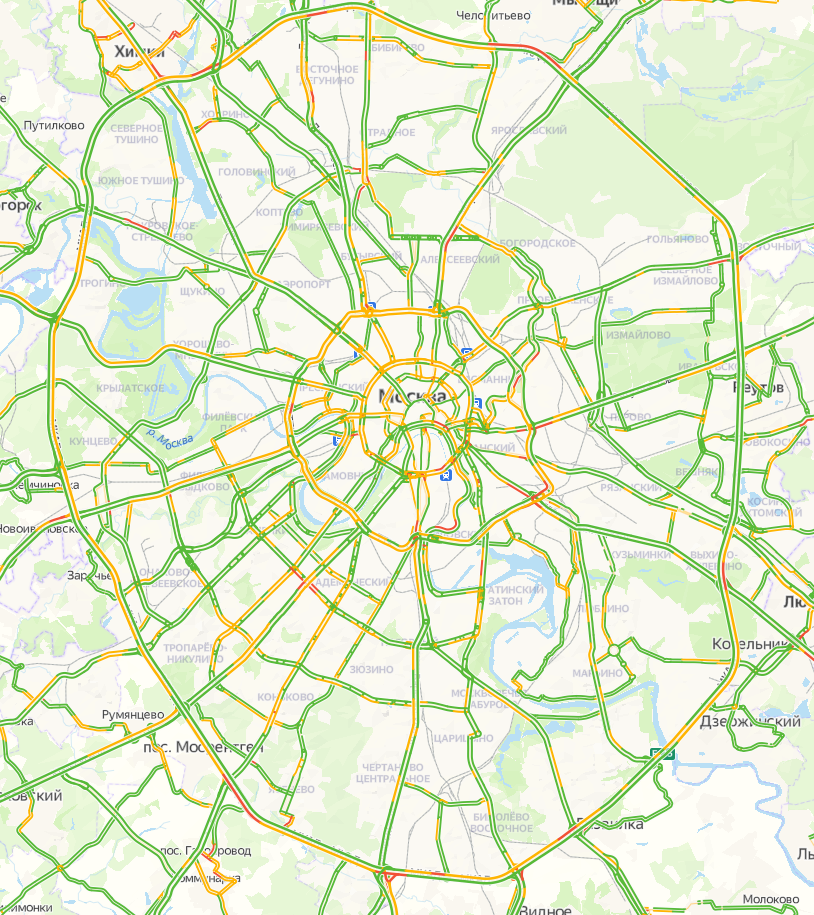
\includegraphics[width=0.5\linewidth]{YandexMap2.png}
        \caption{Типичные пробки по понедельникам в 18:15 на основе статистики сервиса «Яндекс-пробки» транспортной сети Москвы и МКАД, в частности по состоянию на 16.05.21.}
    \end{figure}
\end{frame}

\begin{frame}
    \frametitle{Мотивация к данной работе}
    \begin{itemize}
        \item Планы ЦОДД по управляемому въезду на МКАД,
        \item Микроскопические модели вычислительно тяжёлые,
        \item Макроскопическим моделям возможно не хватает точности;
    \end{itemize}

    Компромисс~--- рассматривать вместо движения каждого отдельного автомобильно-транспортного средства (АТС) движение их групп.
\end{frame}

\section{Математическая модель}
\begin{frame}[plain, noframenumbering]
    \begin{center}
        \Huge
        Математическая модель
    \end{center}
\end{frame}

\subsection{Транспортная сеть}
\begin{frame}
    \frametitle{Транспортная сеть}

    Транспортная сеть представляет собой связный ориентированный граф \(\mathbf{G} = (\mathbf{V}, \mathbf{E})\), где \(\mathbf{V}\) - множество вершин, \(\mathbf{E} = \{(i, j)\}\) - множество ветвей графа.

    Ограничения накладываемые на граф:
    \begin{itemize}
        \item \(\min(d(i)) = 1\),
        \item \(\max(d(i)) = 3\),
        \item \(\forall i: d(i) > 1 \rightarrow \exists j, l \in \mathbf{V} : (j, i), (i, l) \in \mathbf{E}\);
    \end{itemize}
\end{frame}

\subsection{Свойства группы АТС}
\begin{frame}
    \frametitle{Свойства группы АТС}
    Свойства группы АТС на ветви \((i, j): \mathbf{A}^t_k = \{\mathrm{Pos}_k, V_k, N_k\}:\)
    \begin{enumerate}
        \item \(\mathrm{Pos}_k\)~--- позиция начала группы относительно начала ветви на которой она расположена,
        \item \(V_k\)~--- скорость группы АТС,
        \item \(N_k\)~--- размер группы АТС из \(\mathbb{R}_{\geq 0} = \mathbb{R}_+\);
    \end{enumerate}

    Пусть теперь \(\mathbf{A}^t_{i,j} = \{\mathbf{A}^t_k\}\)~--- упорядоченное множество автомобильных групп на ветви \((i,j)\).

    \begin{block}{Состояние системы в момент времени \(t\)}
    \(\mathbf{A}^t = \{\mathbf{A}^t_{i,j}\} \cup \{A^t_{\text{out}, i, j}\}\)
    \end{block}
\end{frame}

\begin{frame}
    \frametitle{Расчёт характеристик группы АТС}
    \begin{enumerate}
      \item Скорость группы рассчитывается на основе плотности автомобилей на ветви автомагистрали и фундаментальной диаграммы поток-плотность.
      \item Длинна группы АТС считается линейно зависящей от ее скорости по формуле \(L = L_\text{avg} + a\cdot V\).
    \end{enumerate}
\end{frame}


\subsection{Процедура расчёта}
\begin{frame}
    \frametitle{Необходимые алгоритмы}
    \begin{itemize}
        \item Движение групп АТС по ветви,
        \item Объединение двух групп АТС,
        \item Перемещение групп АТС между ветвями,
        \item Расчёта потенциала трансфера между ветвями;
    \end{itemize}
\end{frame}

\begin{frame}
    \frametitle{Расчётный цикл}
    \begin{enumerate}
      \item Генерируем АТС всеми источниками в модели.
      \item Движение групп АТС на всех сегментах автомагистрали в порядке удалённости от конца магистрали.
      \item Очистка всех сегментов-стоков в модели от транспортных средств. Возврат к п.1.
    \end{enumerate}
\end{frame}

\section{Фундаментальная диаграмма потока}
\begin{frame}[plain, noframenumbering]
    \begin{center}
        \Huge
        Фундаментальная диаграмма потока
    \end{center}
\end{frame}

\begin{frame}
    \frametitle{Данные дорожных датчиков}
    \begin{figure}[ht]
        \begin{center}
            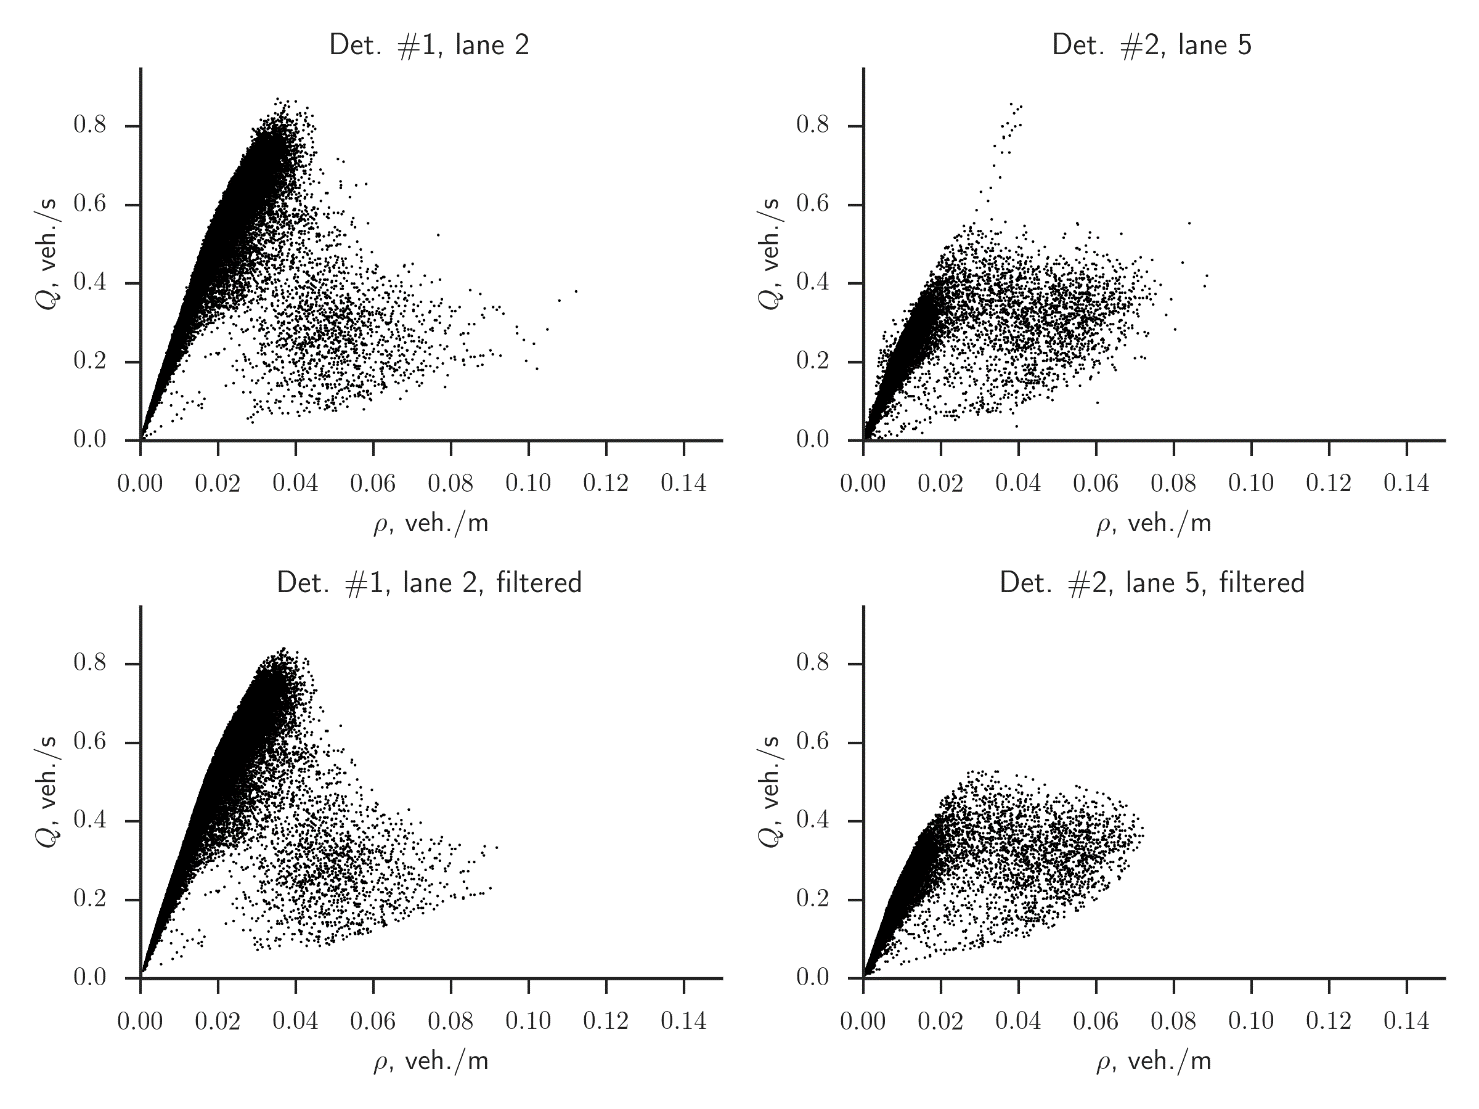
\includegraphics[width=1\linewidth]{detectors_data_alpha.png}
            \caption{Экспериментальные данные с двух детекторов, установленных на различных полосах МКАД --- замеренные интенсивности транспортного потока \(Q(\rho)\)[АТС/с] при различной плотности [АТС/м]. Данные представлены за 2012 г. В количестве 288 измерений за день. Сверху исходные данные, снизу отфильтрованные с использованием алгоритма построения выпуклых оболочек.}
        \end{center}
    \end{figure}
\end{frame}

\begin{frame}
    \frametitle{Три фазы Кернера}
    \begin{enumerate}
      \item Свободный поток \(Q(\rho) = \alpha_2\rho^2 + \alpha_1\rho,\ 0\leq\rho\leq\rho_1\),
      \item Синхронизованный поток \(Q(\rho) = \beta_2\rho^2 + \beta_1\rho + \beta_0,\ \rho_1\leq\rho\leq\rho_2\),
      \item Заторный поток \(Q(\rho) = c_*(\rho_*-\rho),\ \rho_1\leq\rho\leq\rho_*\);
    \end{enumerate}

    Kerner, B. S. Introduction to modern traffic flow theory and control [Текст]. Т. 700 / B. S. Kerner. — Springer, 2009.
\end{frame}

\begin{frame}
    \frametitle{Пример фундаментальных диаграмм}
    \begin{figure}[ht]
        \begin{center}
            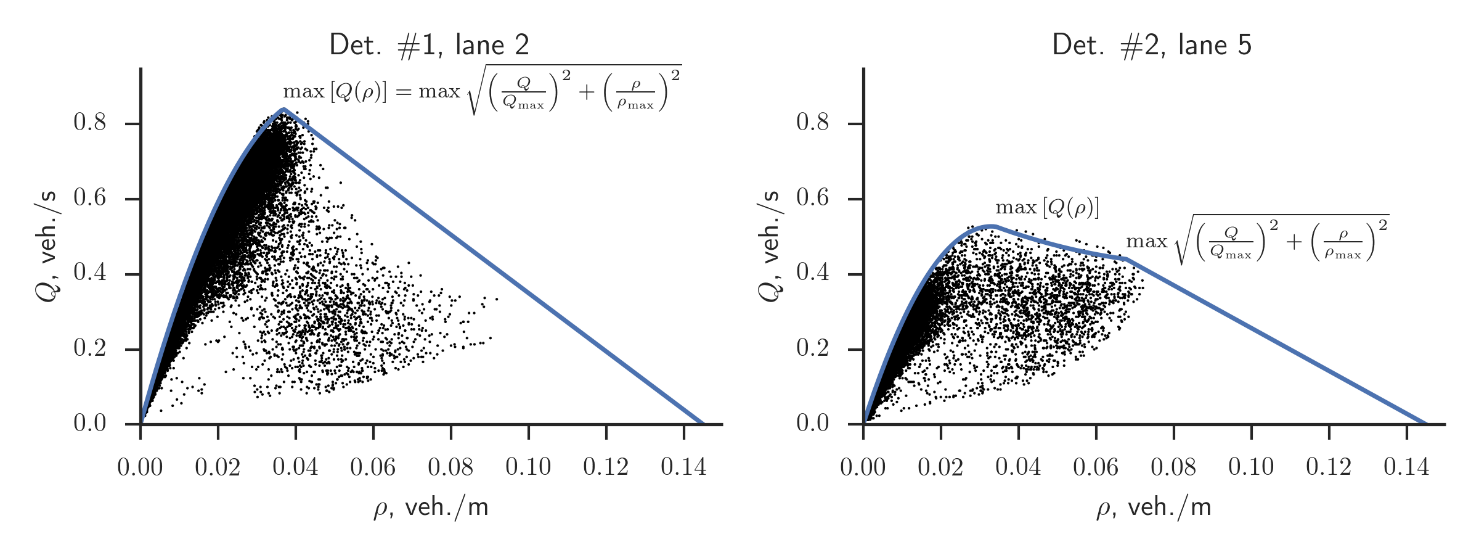
\includegraphics[width=1\linewidth]{Q_result.png}
            \caption{Фундаментальные диаграммы для двух разных участков МКАД. Слева для данных со второй полосы (детектор № 1), справа с пятой полосы (детектор №2)}
        \end{center}
    \end{figure}

\end{frame}

\begin{frame}
    \frametitle{Расчет скорости волны торможения}
    \begin{figure}[ht]
        \begin{center}
            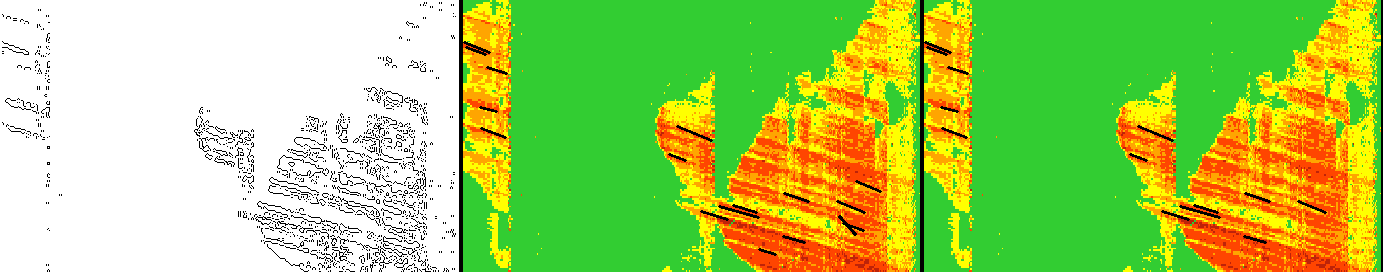
\includegraphics[width=1\linewidth]{c_end.png}
            \caption{Нахождение значений скорости волн торможения на пространственно-временной структуре значений скорости транспортного потока на внешней стороне МКАД}
        \end{center}
    \end{figure}

    Итоговая скорость волны торможения равна \(-15,8\) км/ч.
\end{frame}


\section{Комплексирование данных}
\subsection{Комплексирование данных}
\begin{frame}[plain, noframenumbering]
    \begin{center}
        \Huge
        Комплексирование данных
    \end{center}
\end{frame}

\subsection{Необходимость комплексирования данных}
\begin{frame}
    \frametitle{Необходимость комплексирования данных}
    \begin{enumerate}
      \item Дорожные датчики относительно точны, но не покрывают всю транспортную сеть.
      \item GPS-треки имеют низкую точность, но покрывают большой объём транспортной сети.
    \end{enumerate}
\end{frame}

\subsection{Функциональная зависимость реального числа АТС от трекового}
\begin{frame}
    \frametitle{Функциональная зависимость реального числа АТС от трекового}
    \centering
    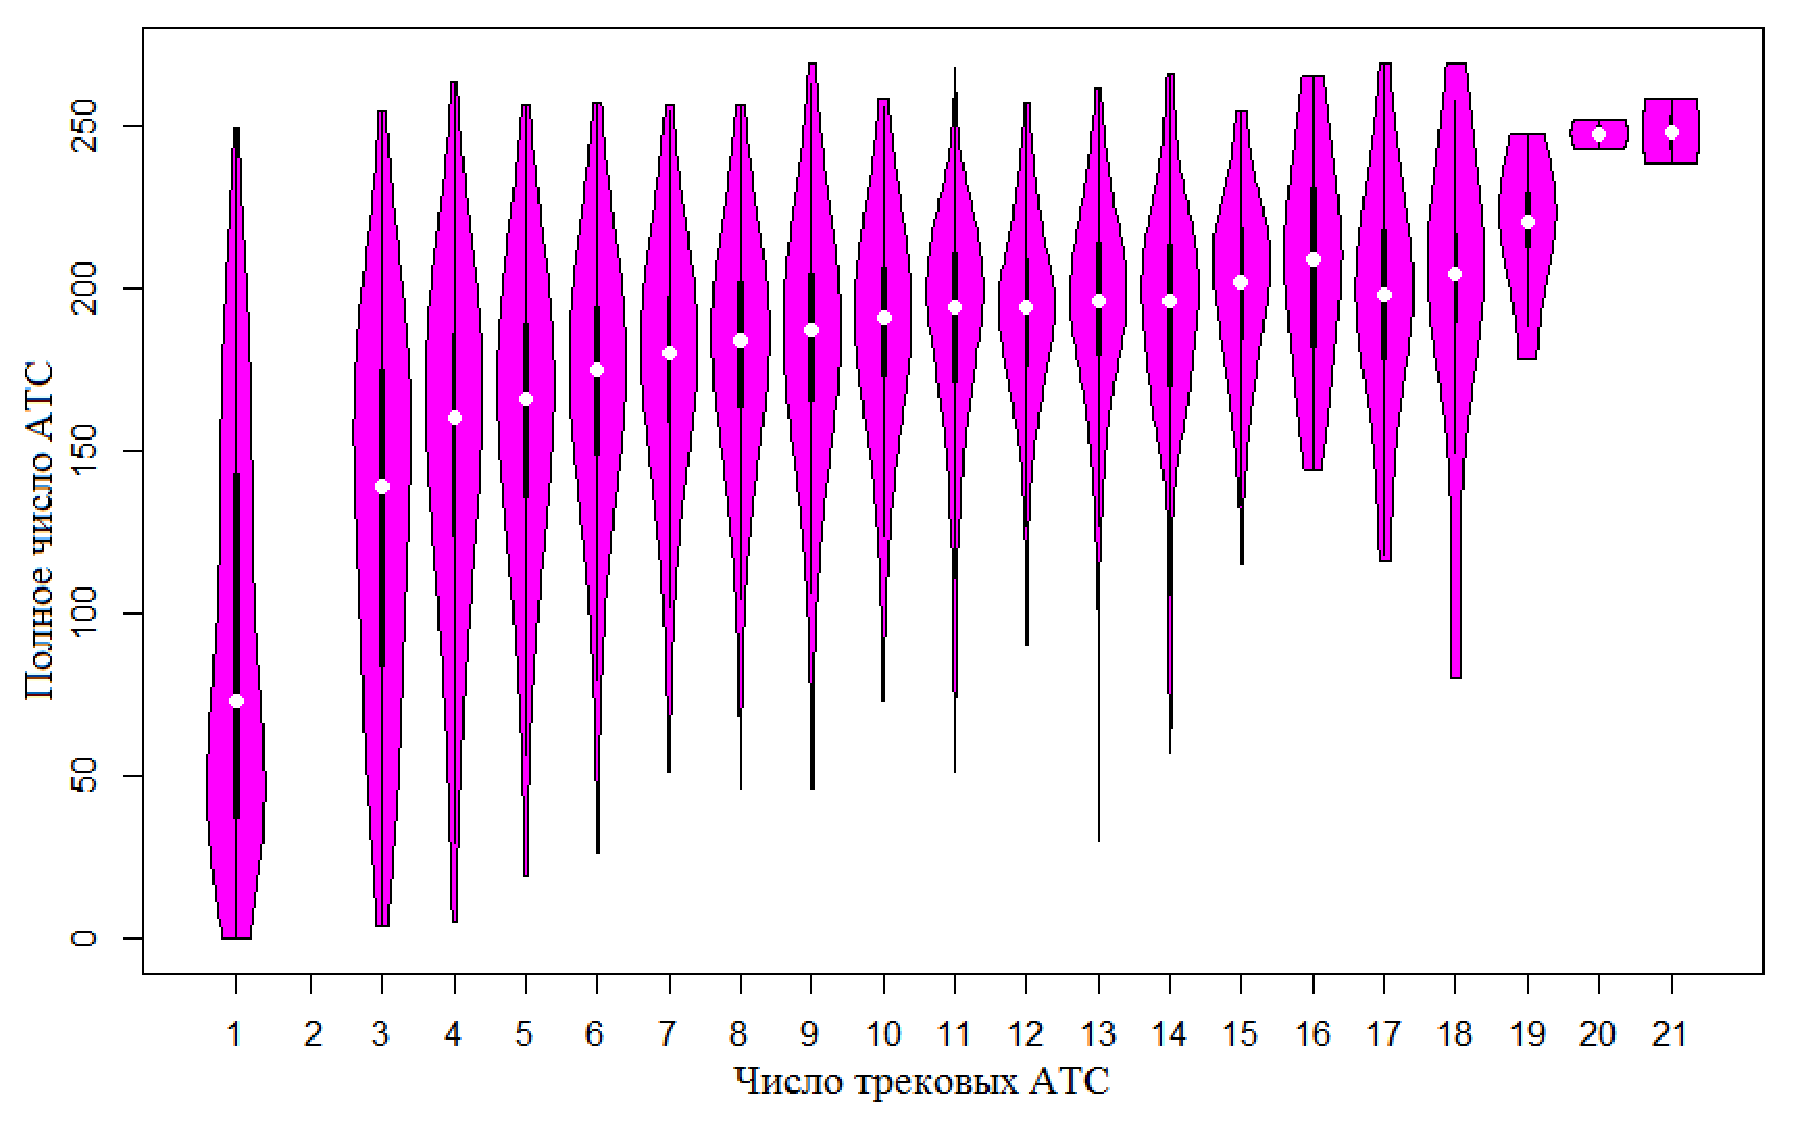
\includegraphics[width=1\linewidth]{Vioplot_Detector-Yandex.eps}
    \begin{equation*}
        \begin{split}
            & N_{\text{real}} = a_0 + a_1N_{\text{track}} + a_2\log\left({N_{\text{track}}}\right) + a_3V + a_4N_{\text{track}}/V
        \end{split}
    \end{equation*}
\end{frame}

\subsection{Преобразование скорости}
\begin{frame}
    \frametitle{Преобразование скорости}
\vspace{-4mm}
\begin{equation*}
    V_{\text{est}} = 12.34 + 0.639V_{\text{track}}
    \label{eq::speed_transform}
\end{equation*}

\vspace{-2mm}
\begin{table}[!ht]
    \centering
    \begin{tabular}{|c|c|c|}
         \hline
         & $V_{\text{est}}$ & $V_{\text{track}}$ \\
         \hline
         Среднеквадратичная ошибка & \textbf{0.03} & 0.042 \\
         \hline
    \end{tabular}
\end{table}
\vspace{-4mm}

    \begin{figure}[!ht]
    \subfloat{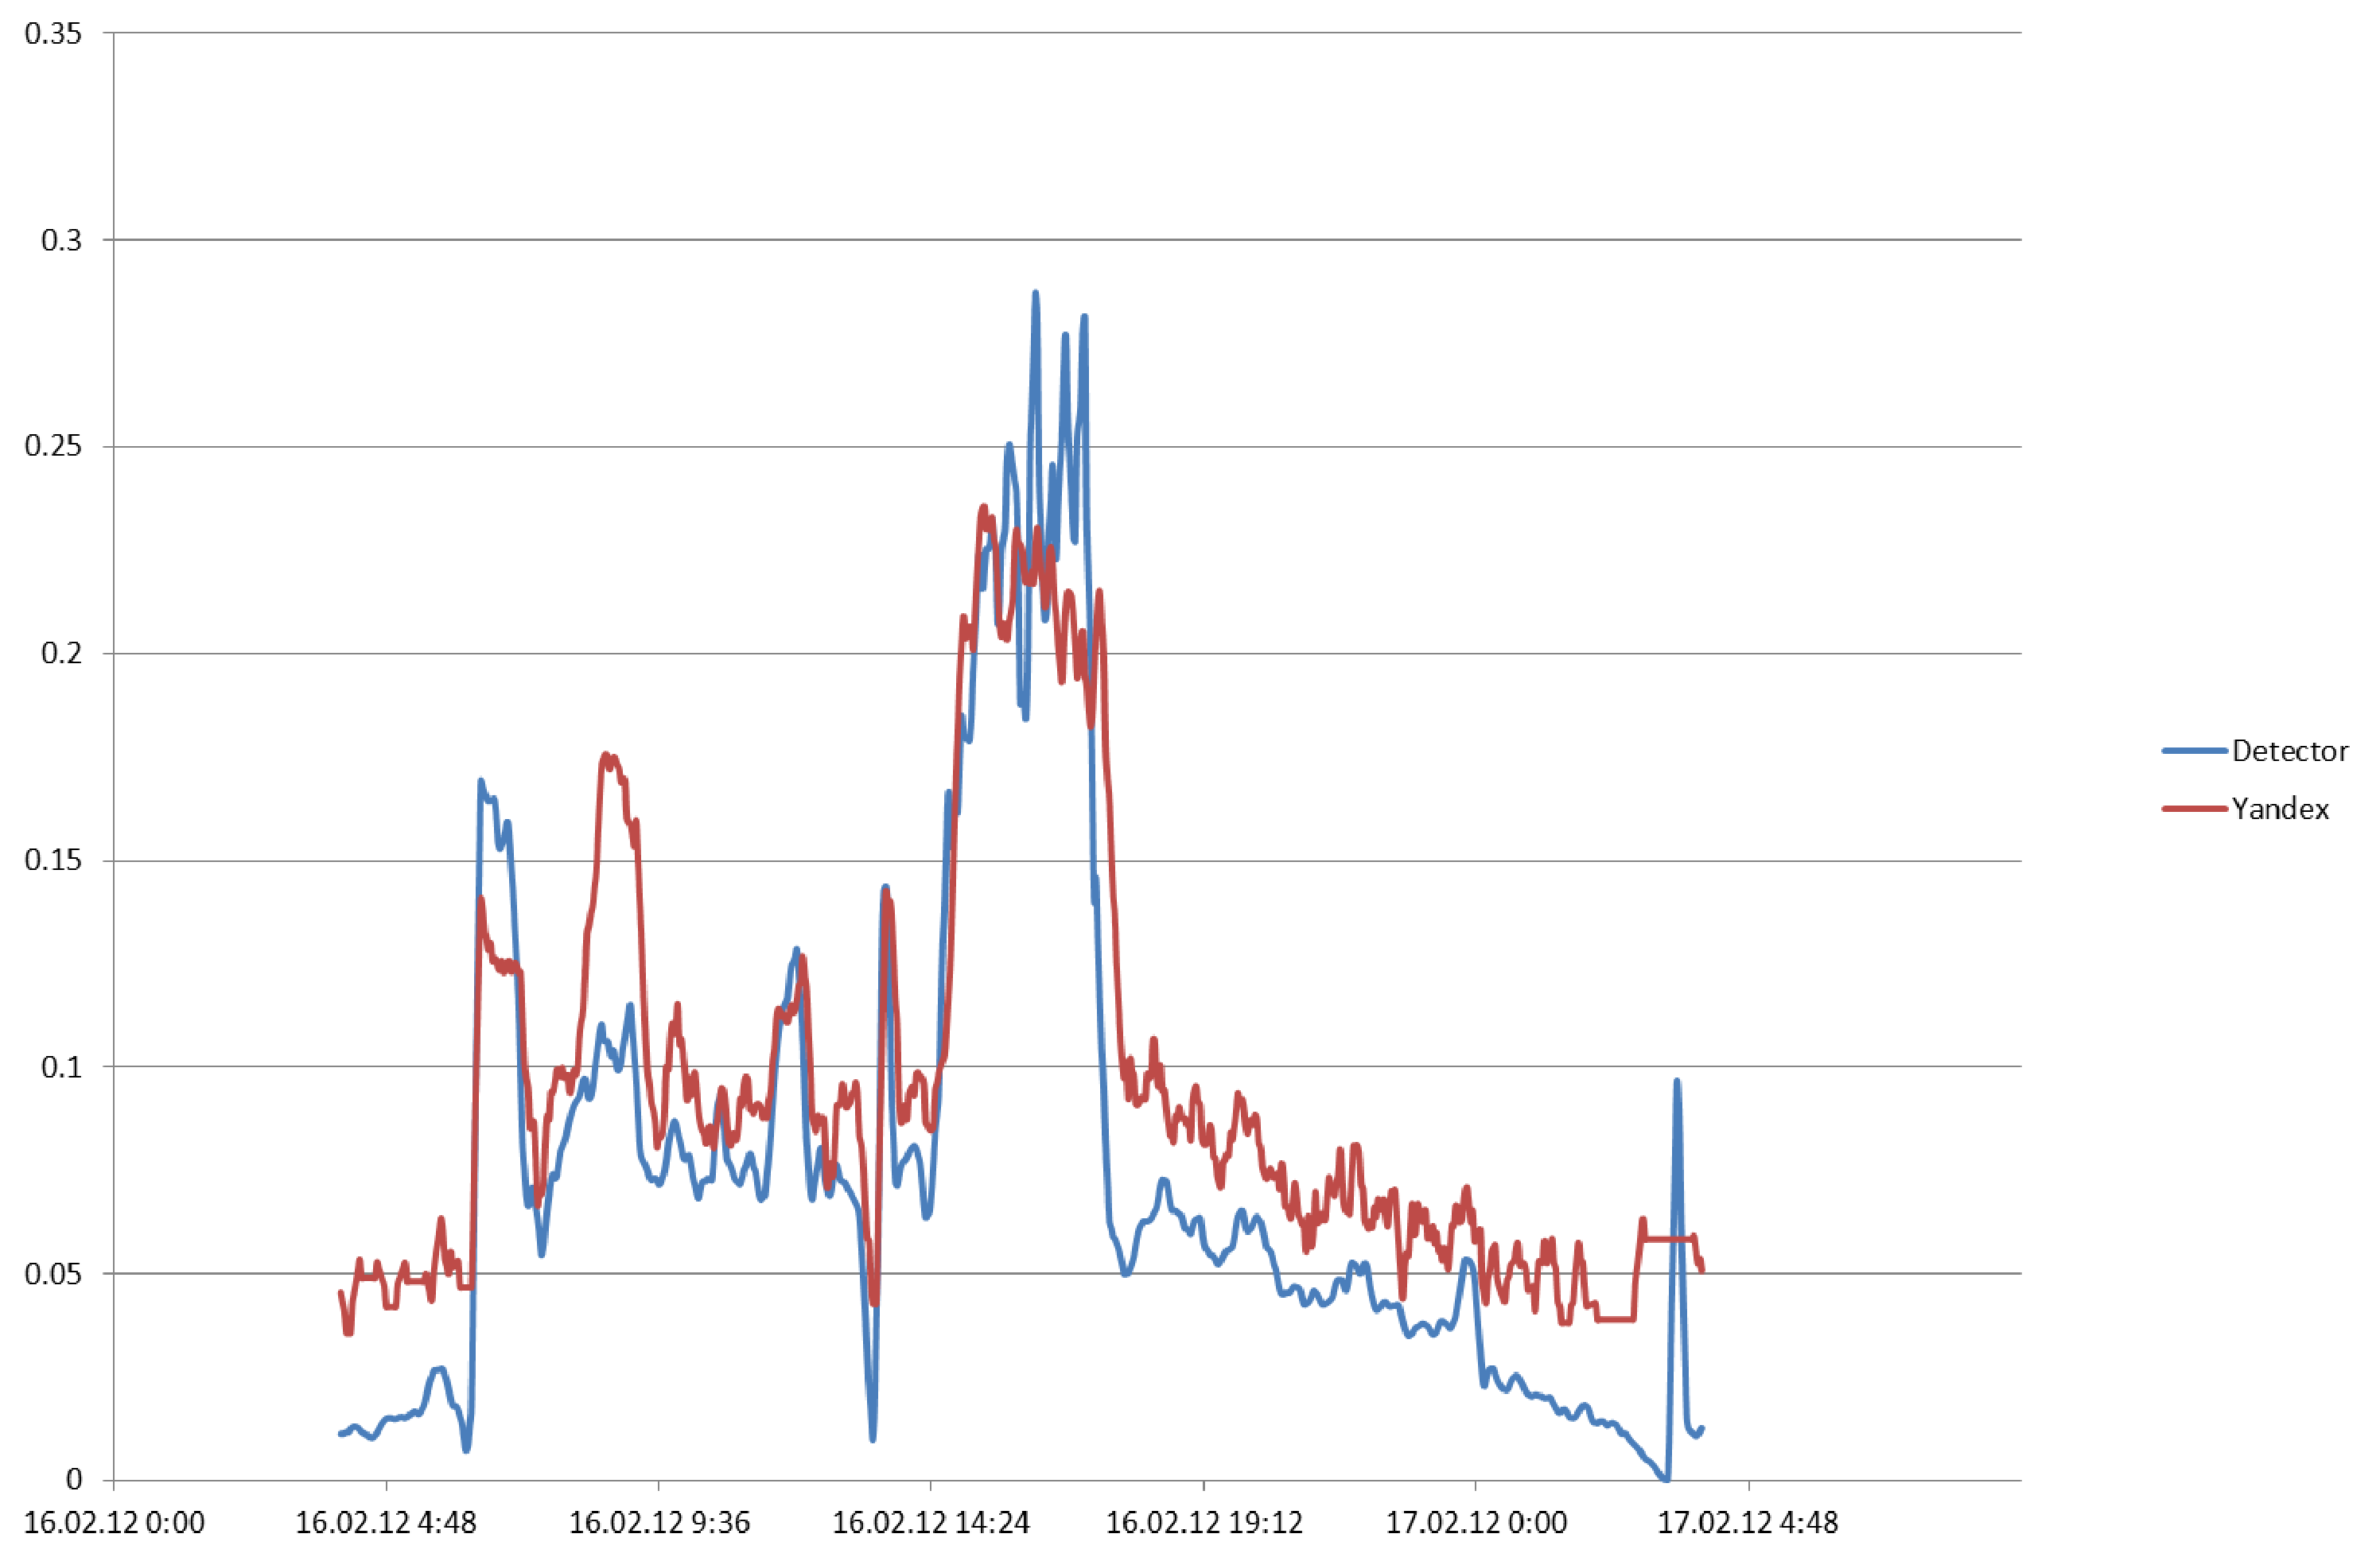
\includegraphics[width=0.45\linewidth]{With_V.eps}}
    \subfloat{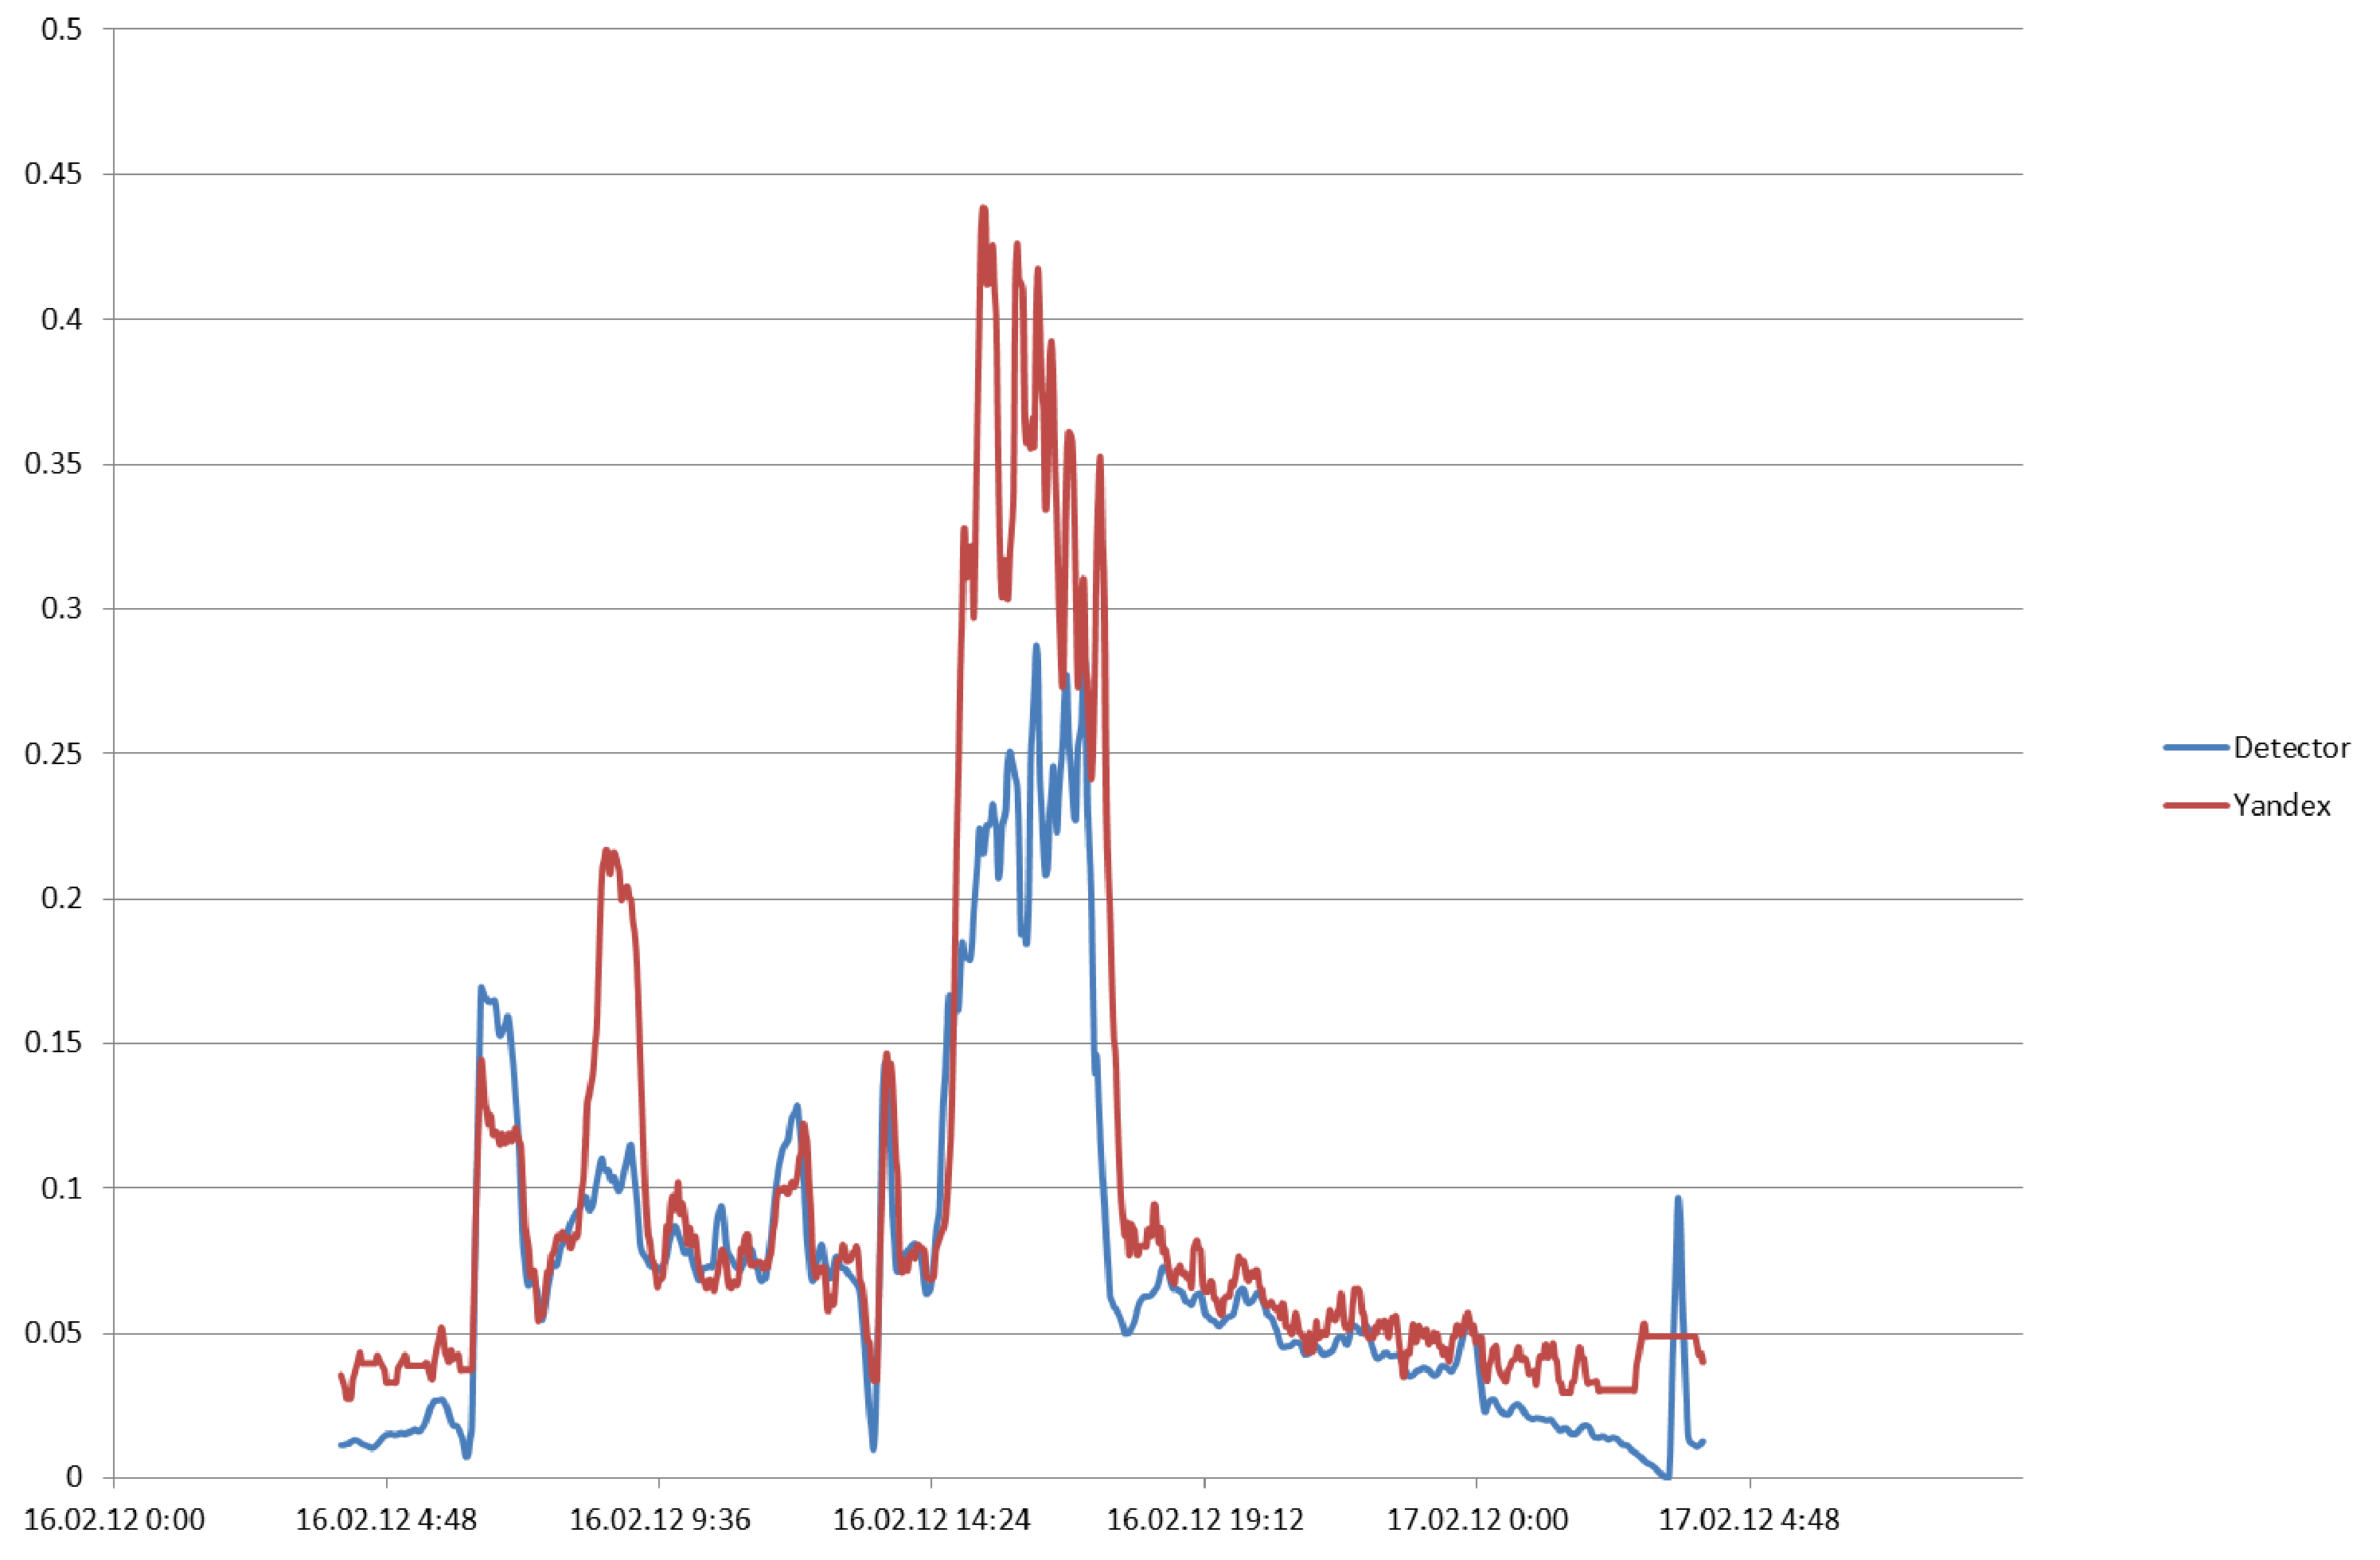
\includegraphics[width=0.45\linewidth]{Without_V.eps}}
    \caption{Восстановленные значения плотности АТС с (слева) и без (справа) преобразования скорости}
    \end{figure}
\end{frame}


\section{Вычислительные эксперименты}
\subsection{Проверка работоспособности модели}
\begin{frame}[plain, noframenumbering]
    \begin{center}
        \Huge
        Проверка работоспособности модели
    \end{center}
\end{frame}

\begin{frame}
    \frametitle{Простая дорога}
  \hfil\hfil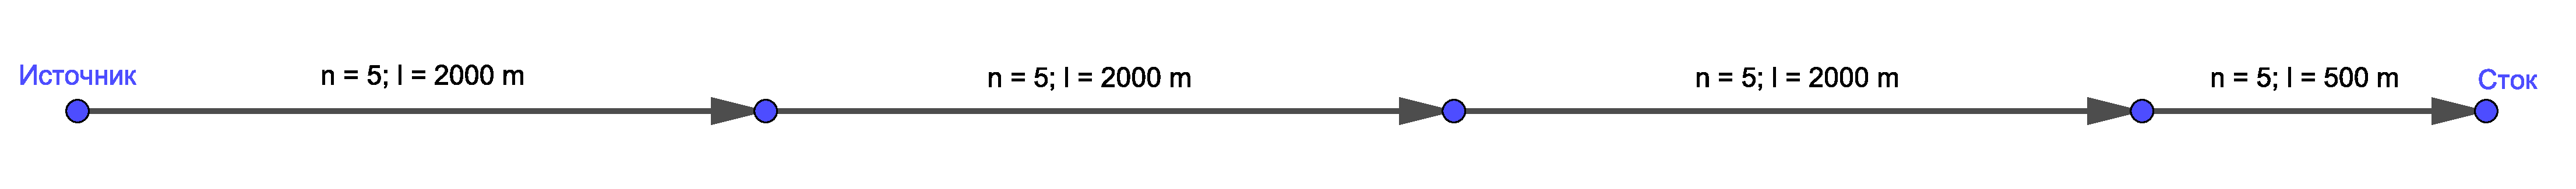
\includegraphics[width=1.0\linewidth]{scheme_simple_3block_road.eps}\newline
  \vfil
  \hfil\hfil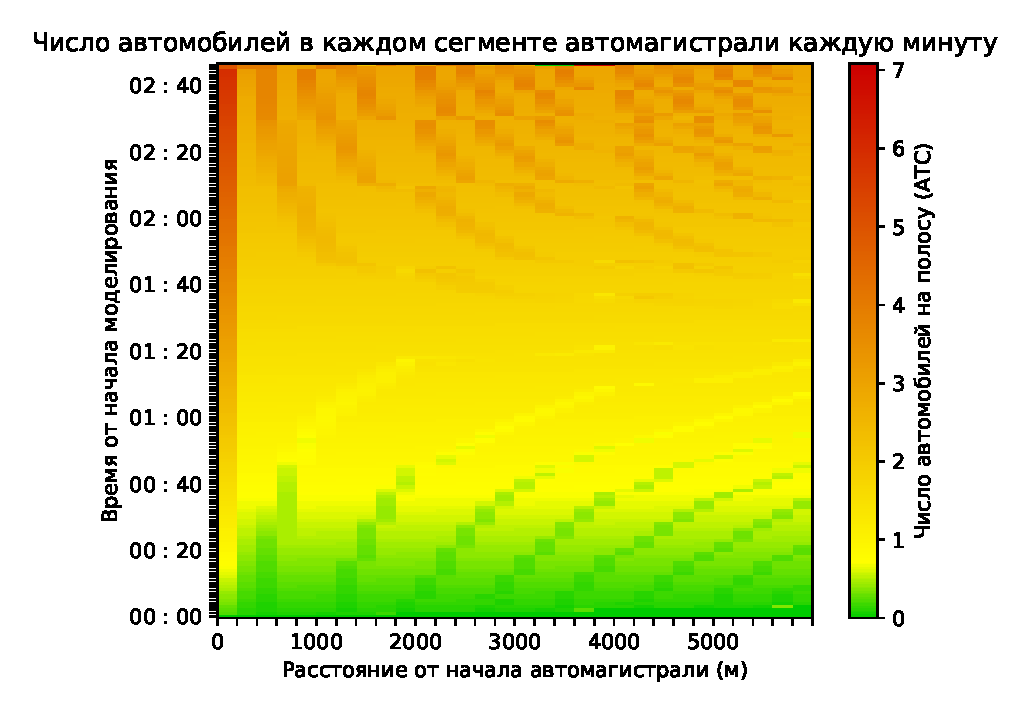
\includegraphics[width=0.5\linewidth]{simple_3_block_road.eps}\hfil\hfil
    \begin{minipage}[b][0.5\textheight][c]{.45\linewidth}
    Простая дорога без перекрестков с линейно нарастающим вплоть до 150 АТС/мин потоком.
    \end{minipage}\newline
\end{frame}

\begin{frame}
    \frametitle{Дорога с сужением, синусоидальный поток}
  \hfil\hfil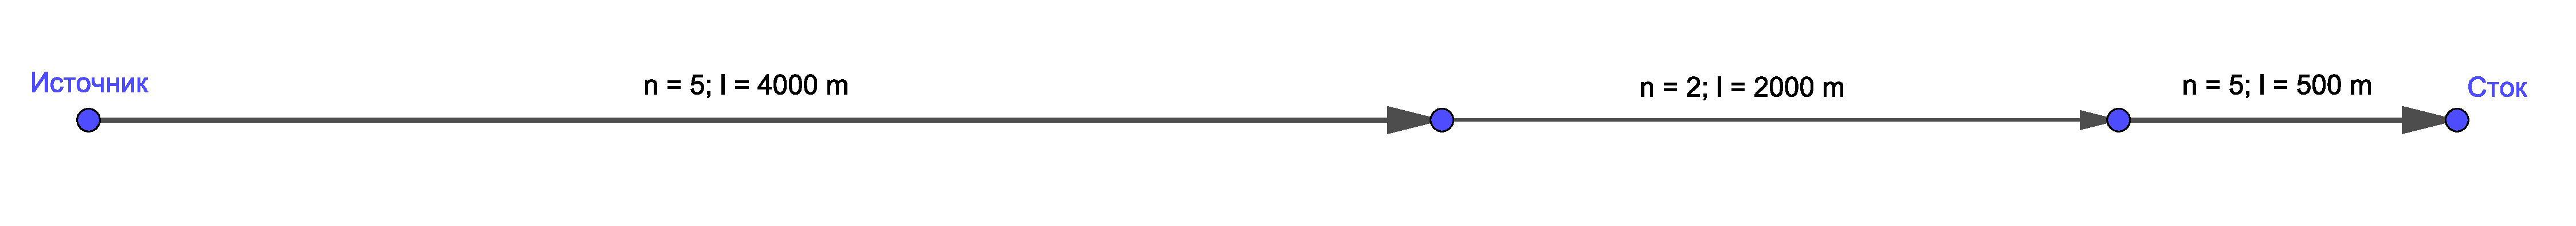
\includegraphics[width=1.0\linewidth]{scheme_jammed_sin_wave.eps}\newline
  \vfil
  \hfil\hfil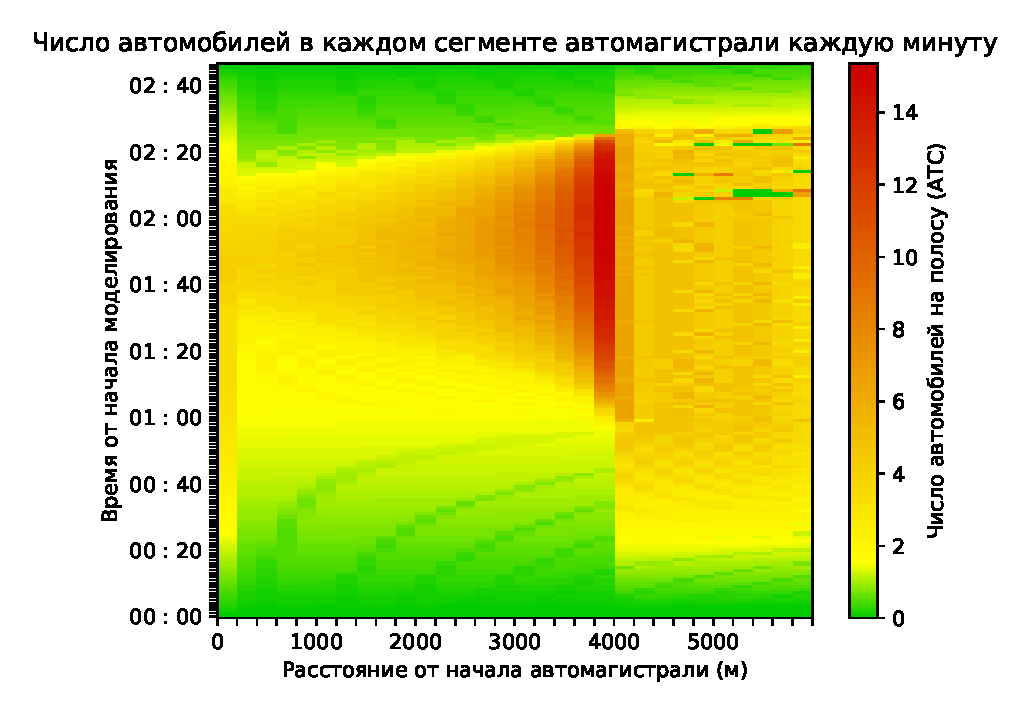
\includegraphics[width=0.5\linewidth]{jammed_5-2_3block_road_sin_wave}\hfil\hfil
    \begin{minipage}[b][0.5\textheight][c]{.45\linewidth}
    Пятиполосная дорога с сужением до двух полос. Входной поток~--- синусоида с периодом равным времени моделирования и амплитудой 85 АТС/мин.
    \end{minipage}\newline
\end{frame}

\begin{frame}
    \frametitle{Дорога с пропадающим сужением}
  \hfil\hfil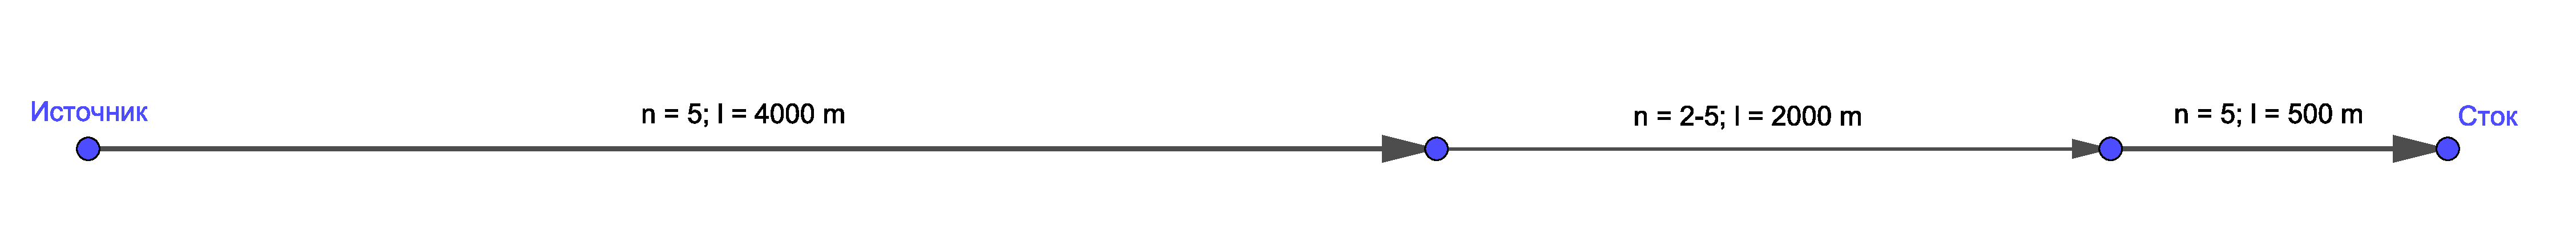
\includegraphics[width=1.0\linewidth]{scheme_jammed_with_unjam.eps}\newline
  \vfil
  \hfil\hfil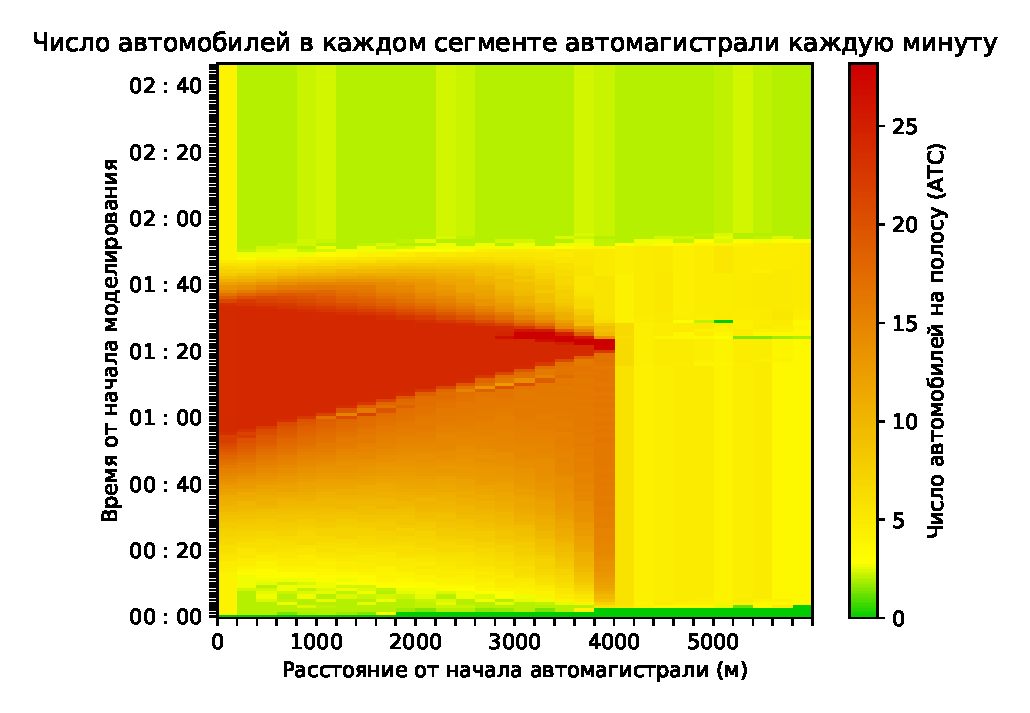
\includegraphics[width=0.5\linewidth]{jammed_5-2_3block_road_with_unjam.eps}\hfil\hfil
    \begin{minipage}[b][0.5\textheight][c]{.45\linewidth}
    Пятиполосная дороге без перекрестков с пропадающим сужением до двух полос. Входной поток 100 АТС/мин.
    \end{minipage}\newline
\end{frame}

\begin{frame}
    \frametitle{Съезд}
  \hfil\hfil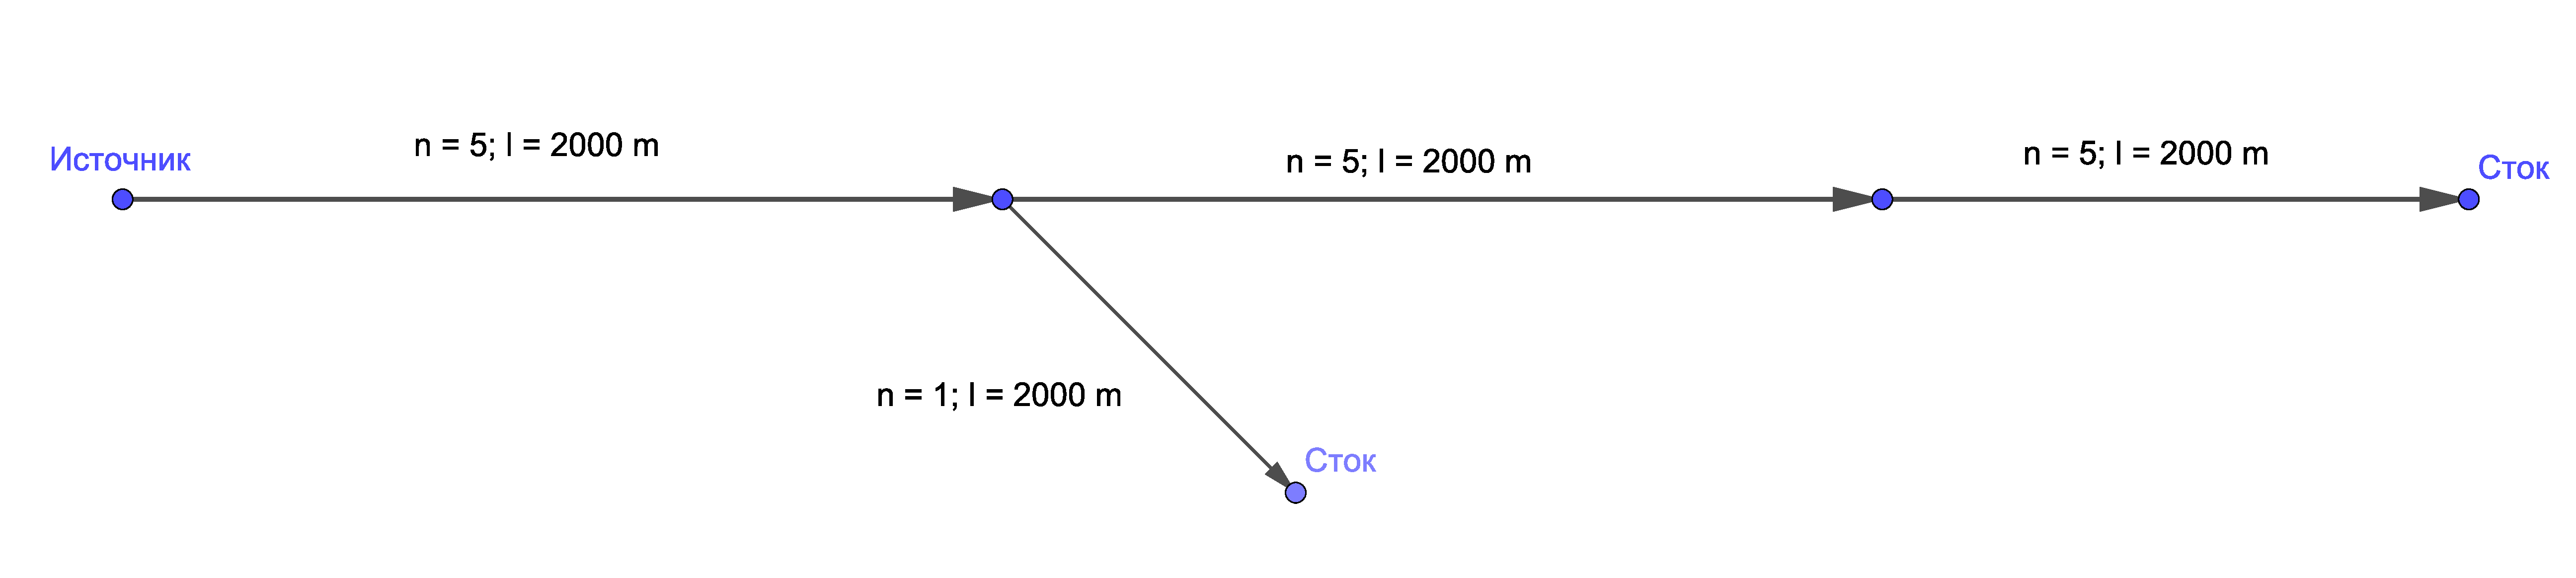
\includegraphics[width=1.0\linewidth]{scheme_jammed_crossroad_exit.eps}\newline
  \vfil
  \hfil\hfil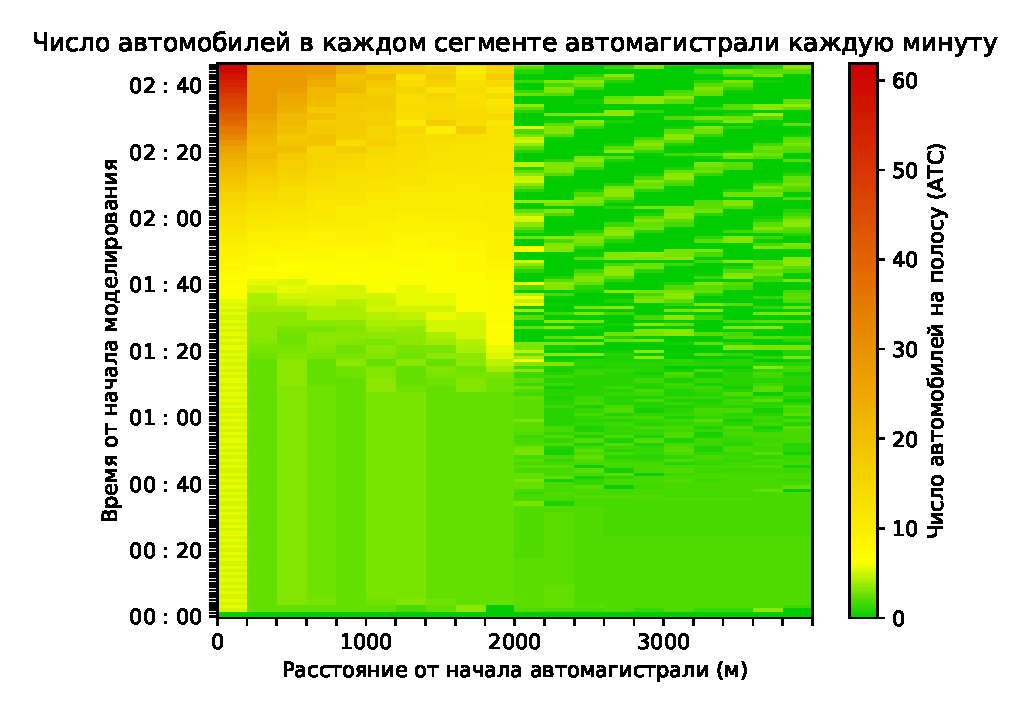
\includegraphics[width=0.5\linewidth]{jamming_crossroad_exit_5_1.eps}\hfil\hfil
    \begin{minipage}[b][0.5\textheight][c]{.45\linewidth}
    Пятиполосная дорога со съездом. Поток на автомагистрали 65 АТС/мин с линейно нарастающей долей съезжающих автомобилей с 20\% до 60\%.
    \end{minipage}\newline
\end{frame}

\begin{frame}
    \frametitle{Въезд}
  \hfil\hfil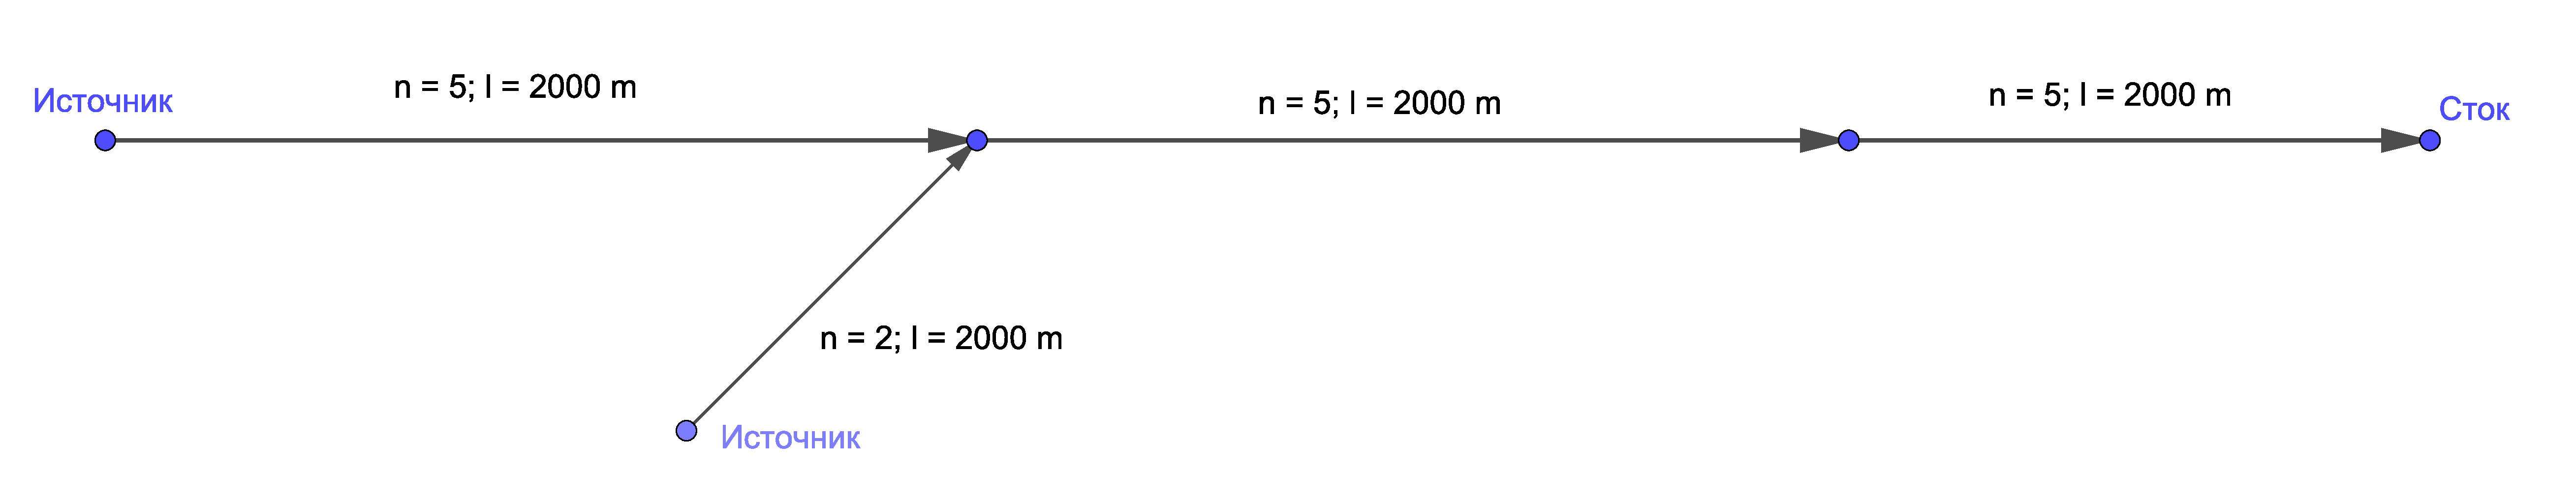
\includegraphics[width=1.0\linewidth]{scheme_jammed_crossroad_enter.eps}\newline
  \vfil
  \hfil\hfil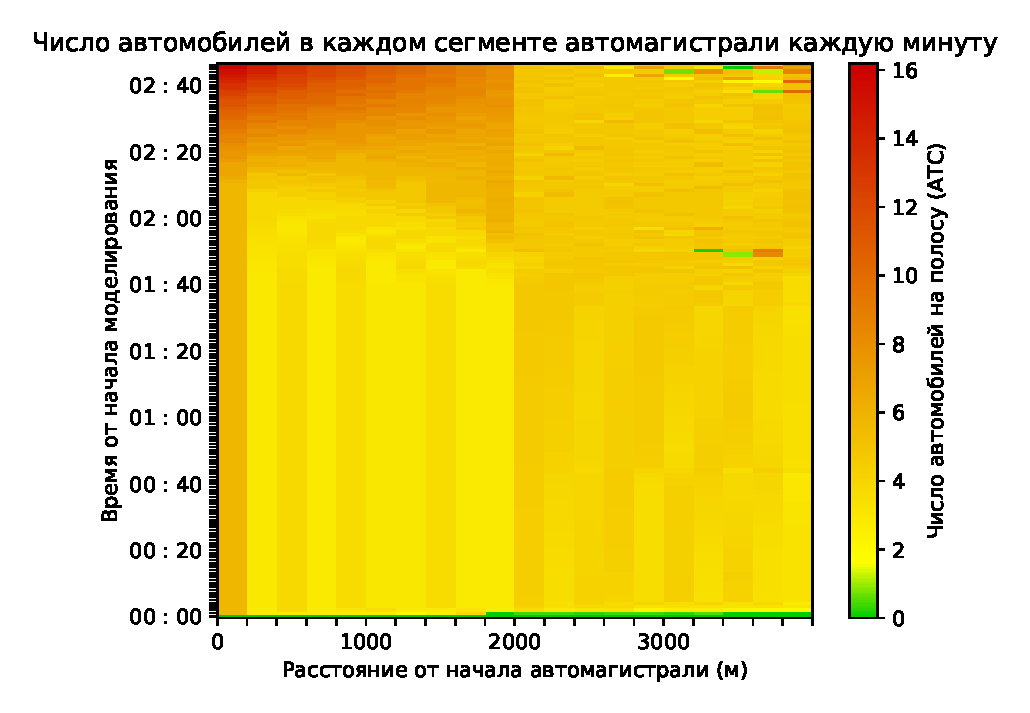
\includegraphics[width=0.5\linewidth]{jamming_crossroad_enter_5_2.eps}\hfil\hfil
    \begin{minipage}[b][0.5\textheight][c]{.45\linewidth}
    Пятиполосная дорога с въездом. Поток на автомагистрали 140 АТС/мин, поток на въезде линейно растет с 20 до 50 АТС/мин.
    \end{minipage}\newline
\end{frame}

\begin{frame}
    \frametitle{Прямая дорога между дорожными датчиками}
    \begin{figure}[h]
        \centering
        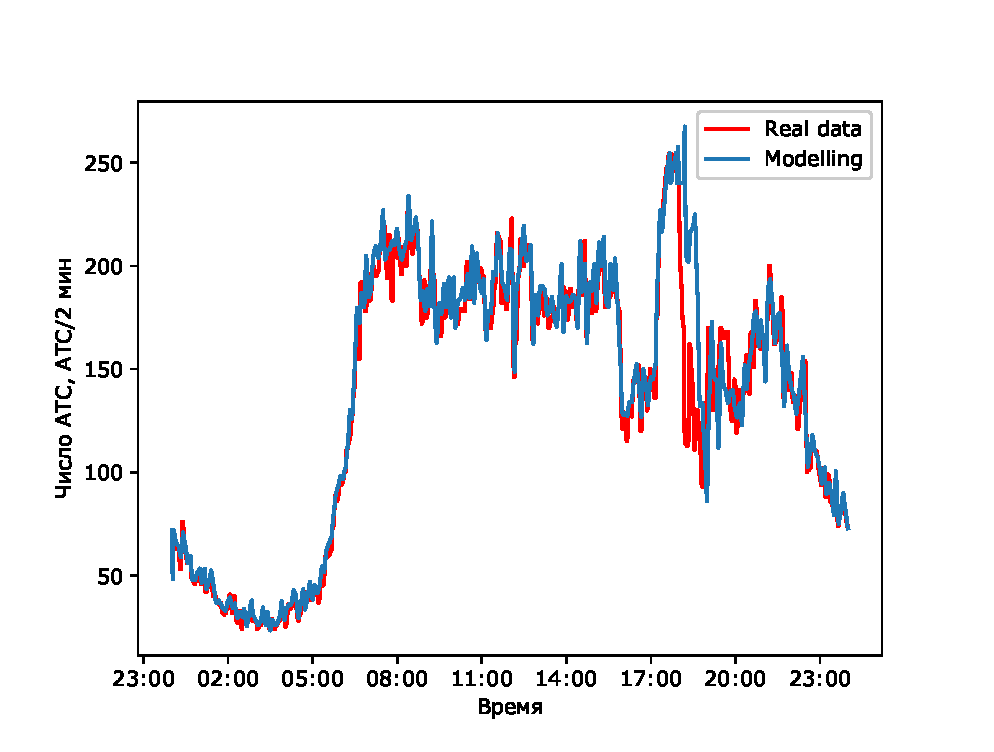
\includegraphics[width=0.6\linewidth]{MCAR_simple_test.eps}
        \caption{График полученного с помощью модели числа съехавших АТС (красная линия) в сравнении с числом съехавших АТС зафиксированных дорожным датчиком (синяя линия) за один день. Среднеквадратичная ошибка $S = 18.4$.}
    \end{figure}
\end{frame}

\begin{frame}
    \frametitle{Прямая дорога между дорожными датчиками. Перекрытая полоса}
    \begin{figure}[ht]
        \centering
        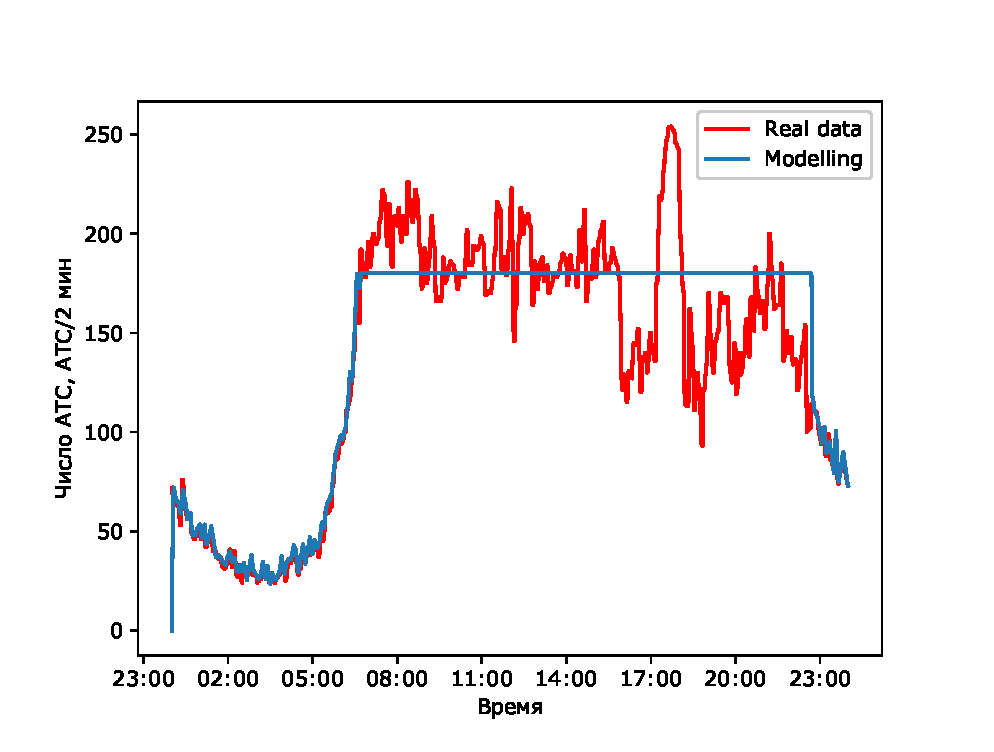
\includegraphics[width=0.6\linewidth]{MCAR_minus_line.eps}
        \caption{График полученного с помощью модели числа съехавших АТС (красная линия) в сравнении с числом съехавших АТС зафиксированных дорожным датчиком (синяя линия) за один день с перекрытием полосы.}
    \end{figure}
\end{frame}



\subsection{Моделирование МКАД}
\begin{frame}[plain, noframenumbering]
    \begin{center}
        \Huge
        Моделирование МКАД
    \end{center}
\end{frame}

\begin{frame}
    \frametitle{Дорожный датчик на въезде}
    \begin{figure}[ht]
    \centering
    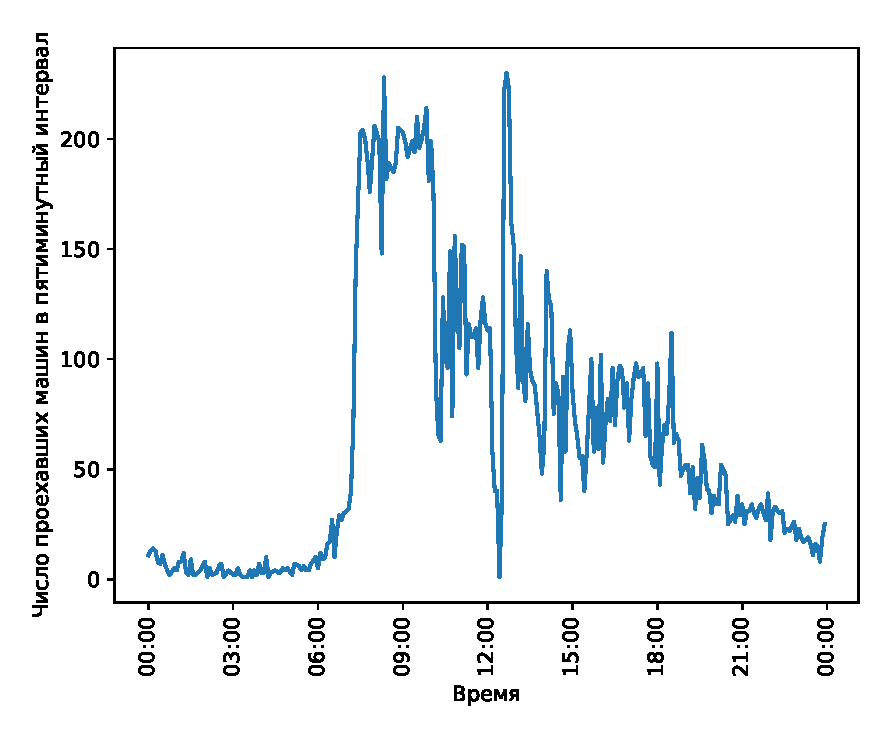
\includegraphics[width=0.6\linewidth]{Detector.eps}
    \caption{Данные с дорожного датчика за один день. Пиковая нагрузка 45 АТС/мин в 8:20.}
\end{figure}
\end{frame}

\begin{frame}
    \frametitle{Входной поток}
    \centering
    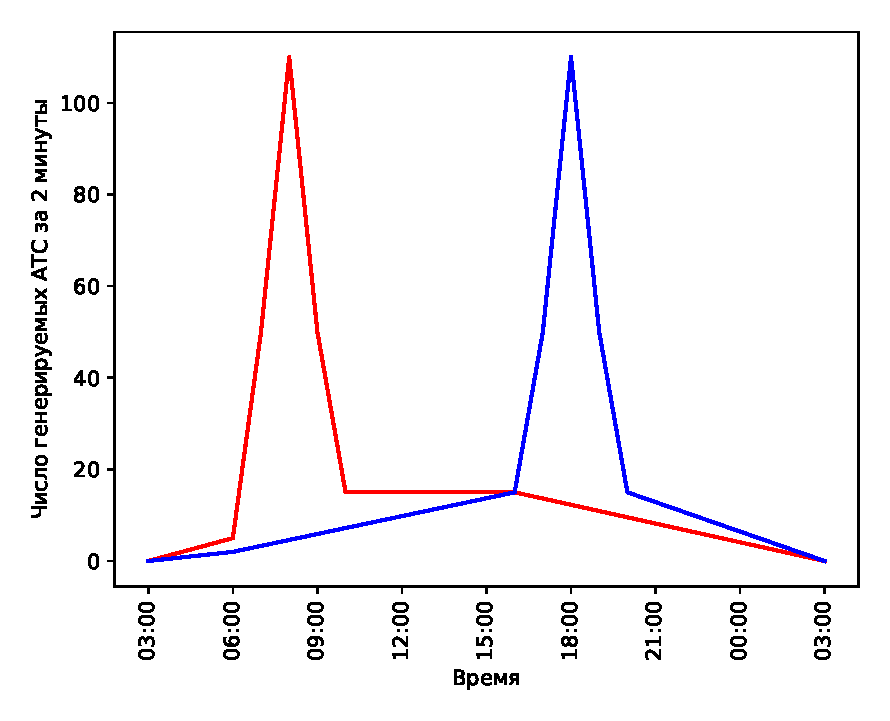
\includegraphics[width=0.75\linewidth]{MCAR_full_woenters_12_two_types_110_24h_3h_Enters_generators.eps} \\
    \hfill
    Графики загрузки двух типов въездов~--- с утренней и вечерней пиковыми загрузками
\end{frame}


\subsubsection{Обычные въезды}
\begin{frame}
    \frametitle{Число автомобилей на автомагистрали}
    \centering
    \begin{minipage}[b]{0.49\textwidth}
        \centering
        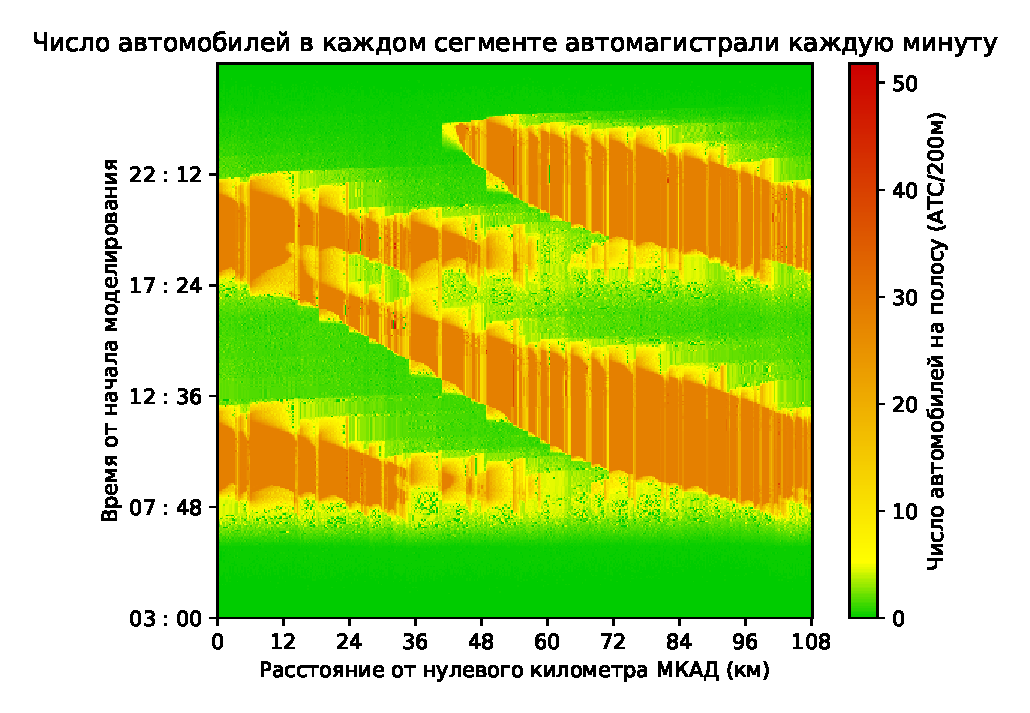
\includegraphics[width=1\linewidth]{MCAR_full_woenters_12_two_types_110_24h_3h.eps}  \\ а) Без управления въездами
    \end{minipage}
    \hfill
    \begin{minipage}[b]{0.49\textwidth}
        \centering
        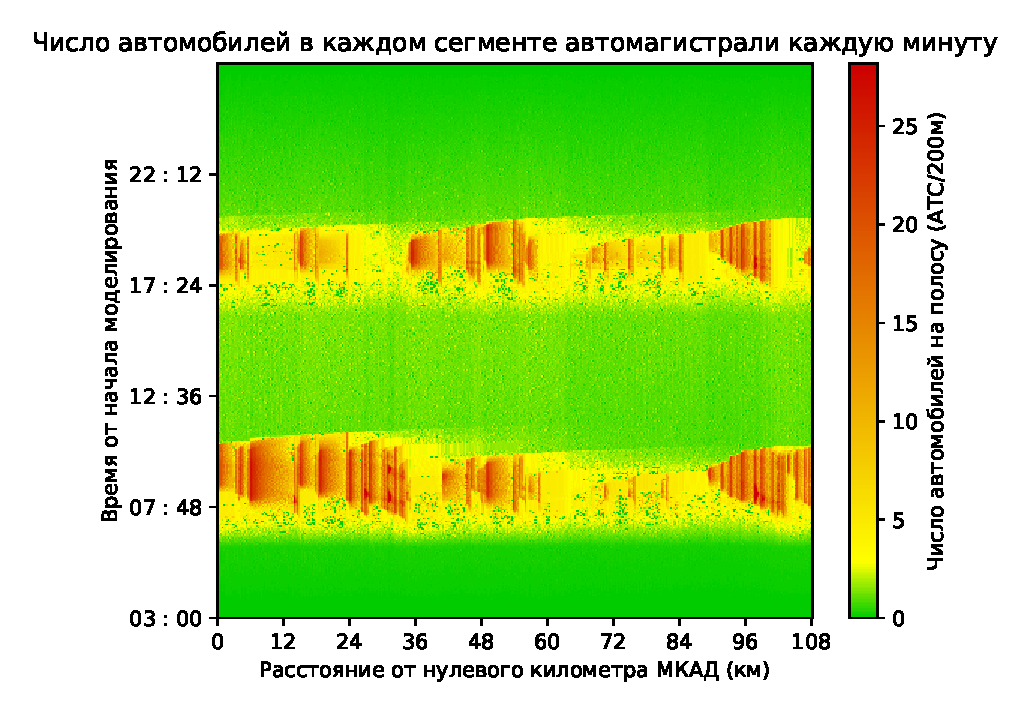
\includegraphics[width=1\linewidth]{MCAR_full_woenters_12_two_types_110_24h_3h_handcontrol.eps}  \\ b) С управлением въездами
    \end{minipage}
    \hfill
    Количество автомобилей на 200 метров в модели транспортной сети МКАД за день
\end{frame}


\begin{frame}
    \frametitle{Число въехавших автомобилей}
    \centering
    \begin{minipage}[b]{.49\textwidth}
        \centering
        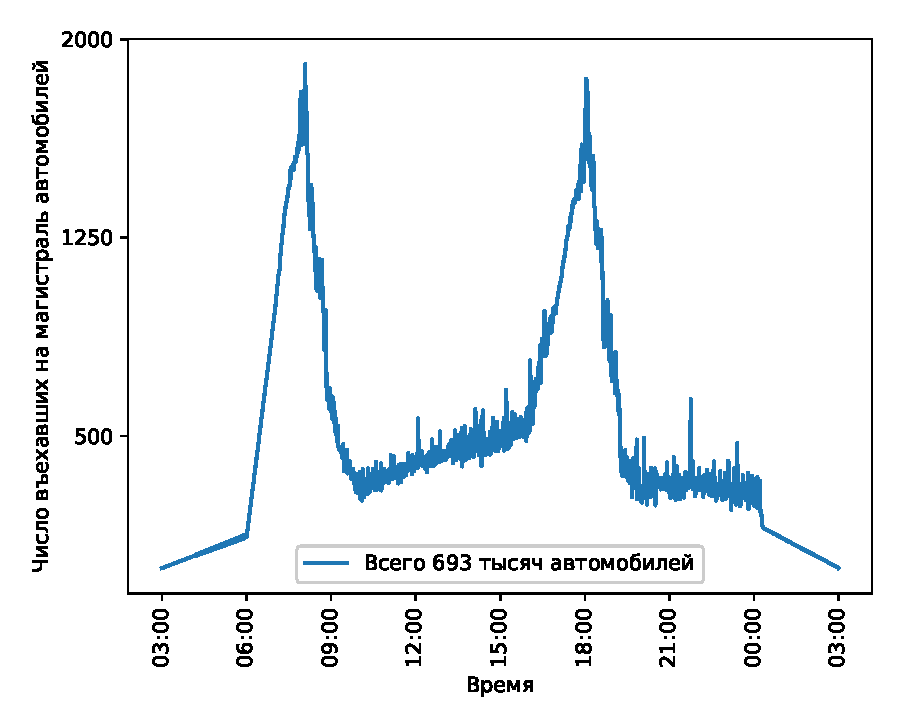
\includegraphics[width=1\linewidth]{MCAR_full_woenters_12_two_types_110_24h_3h_Entered.eps}  \\ а) Без управления въездами
    \end{minipage}
    \hfill
    \begin{minipage}[b]{.49\textwidth}
        \centering
        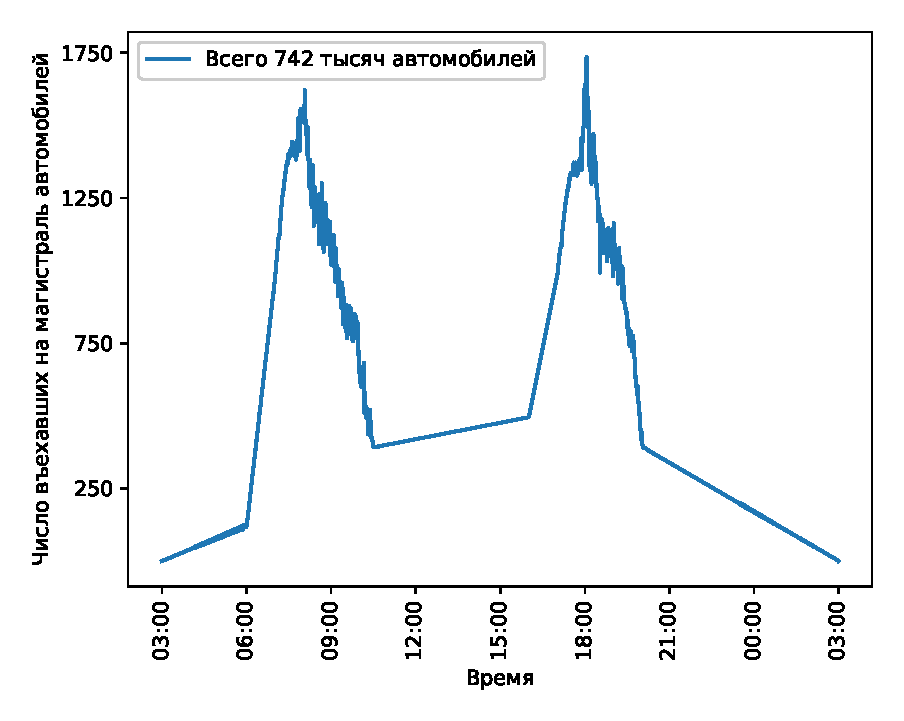
\includegraphics[width=1\linewidth]{MCAR_full_woenters_12_two_types_110_24h_3h_handcontrol_Entered.eps}  \\ b) С управлением въездами
    \end{minipage}
    \hfill
    Графики суммарно въехавшего на МКАД со всех въездов числа автомобилей
\end{frame}


\begin{frame}
    \frametitle{Временные потери на проезд по МКАД}
    \centering
    \begin{minipage}[b]{.49\textwidth}
        \centering
        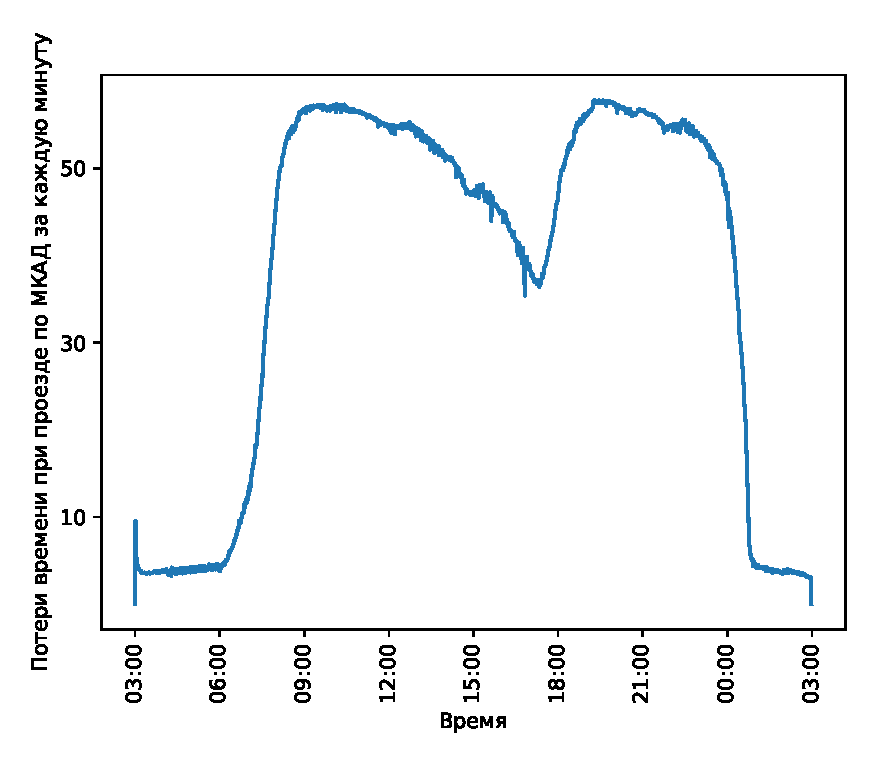
\includegraphics[width=1\linewidth]{MCAR_full_woenters_12_two_types_110_24h_3h_Time_to_pass.eps}  \\ а) Без управления въездами
    \end{minipage}
    \hfill
    \begin{minipage}[b]{.49\textwidth}
        \centering
        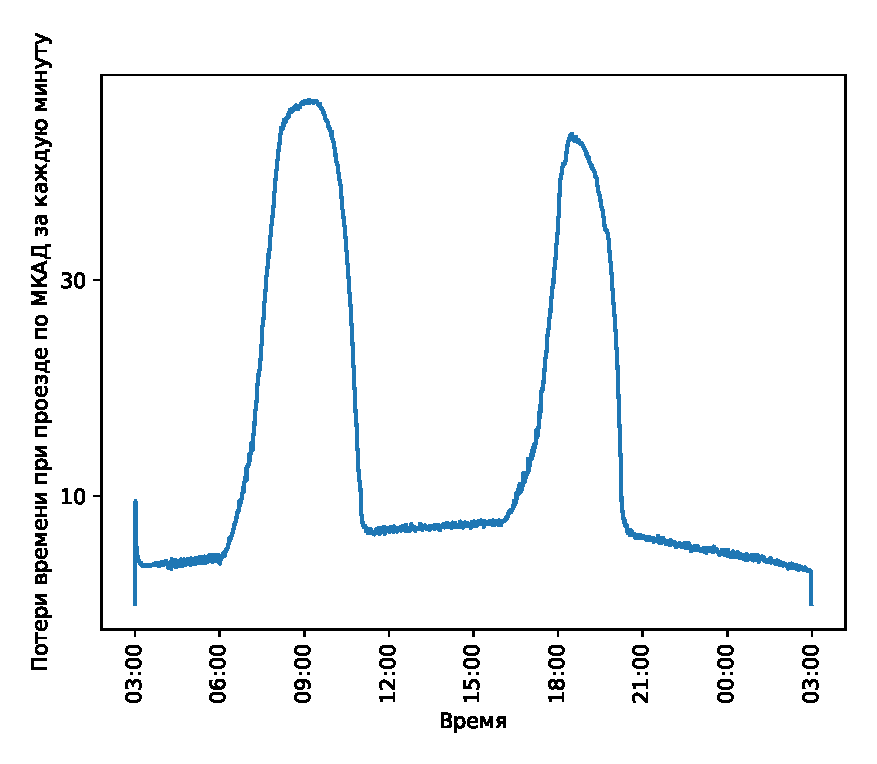
\includegraphics[width=1\linewidth]{MCAR_full_woenters_12_two_types_110_24h_3h_handcontrol_Time_to_pass.eps}  \\ b) С управлением въездами
    \end{minipage}
    \hfill
    Временные потери на проезд по МКАД относительно пустой автомагистрали
\end{frame}

\subsubsection{Длинные въезды}
\begin{frame}
    \frametitle{Число автомобилей на автомагистрали}
    \centering
    \begin{minipage}[b]{0.49\textwidth}
        \centering
        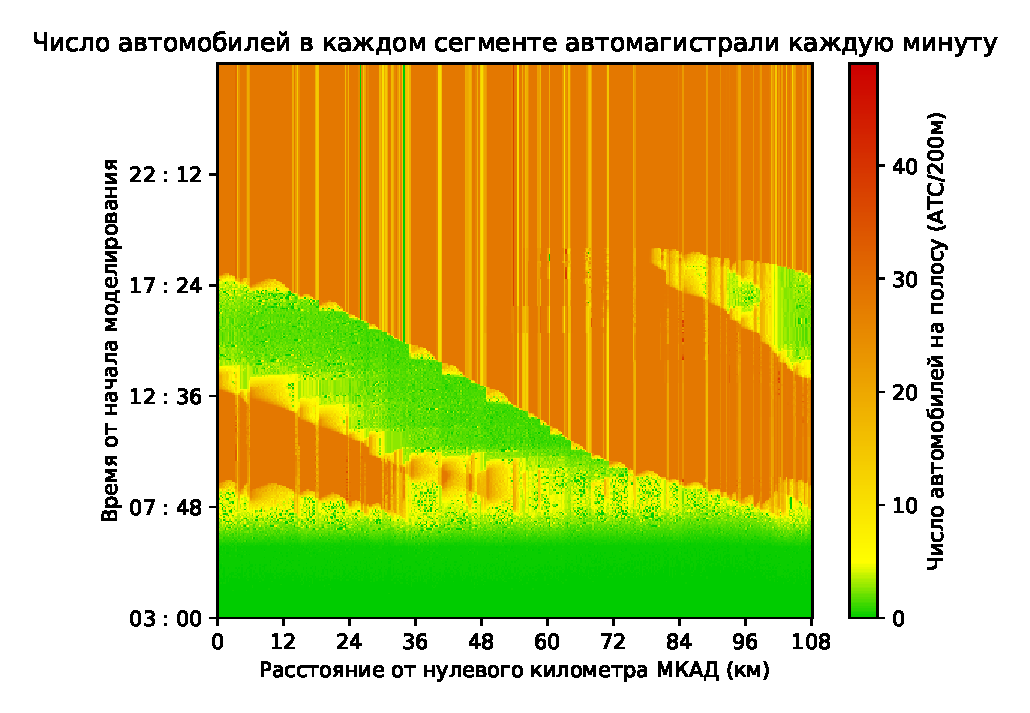
\includegraphics[width=1\linewidth]{MCAR_full_woenters_12_two_types_110_24h_3h_6km.eps}  \\ а) Без управления въездами
    \end{minipage}
    \hfill
    \begin{minipage}[b]{0.49\textwidth}
        \centering
        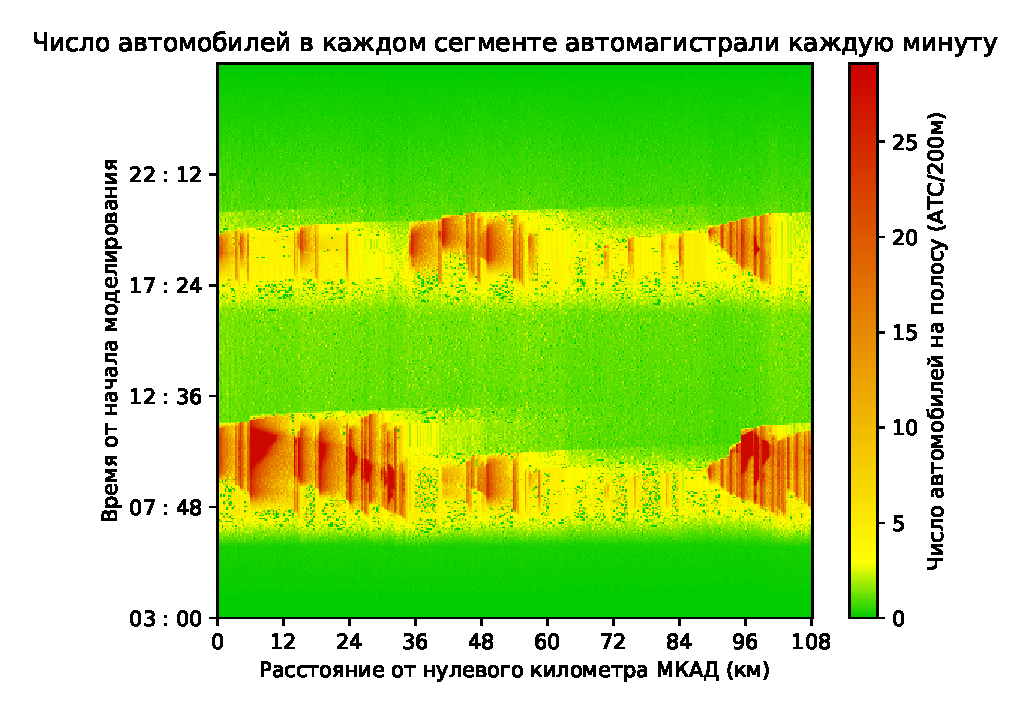
\includegraphics[width=1\linewidth]{MCAR_full_woenters_12_two_types_110_24h_3h_6km_handcontrol.eps}  \\ b) С управлением въездами
    \end{minipage}
    \hfill
    Количество автомобилей на 200 метров в модели транспортной сети МКАД за день
\end{frame}


\begin{frame}
    \frametitle{Число въехавших автомобилей}
    \centering
    \begin{minipage}[b]{.49\textwidth}
        \centering
        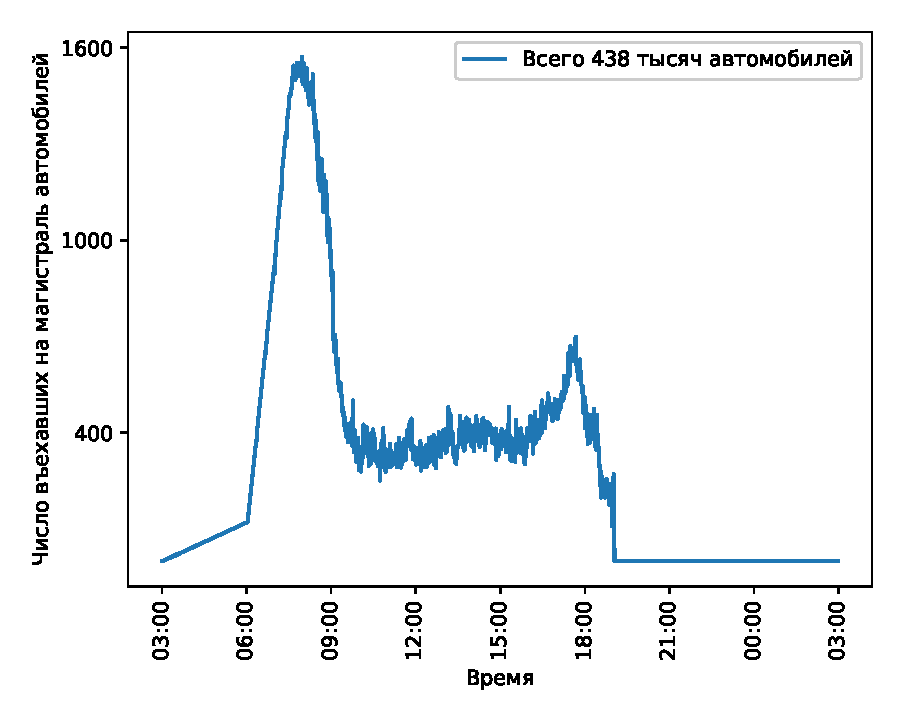
\includegraphics[width=1\linewidth]{MCAR_full_woenters_12_two_types_110_24h_3h_6km_Entered.eps}  \\ а) Без управления въездами
    \end{minipage}
    \hfill
    \begin{minipage}[b]{.49\textwidth}
        \centering
        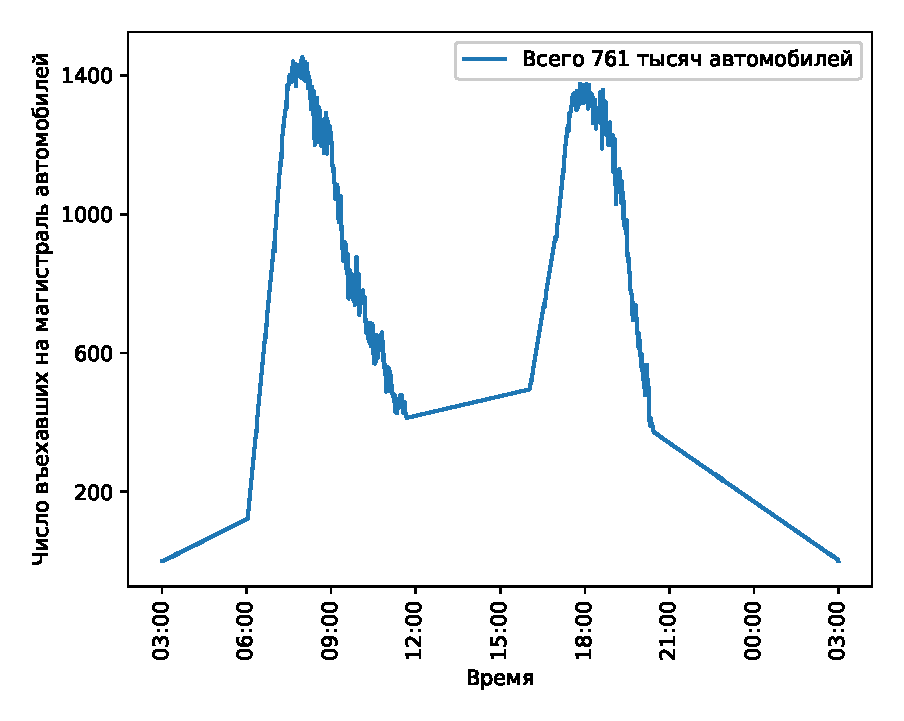
\includegraphics[width=1\linewidth]{MCAR_full_woenters_12_two_types_110_24h_3h_6km_handcontrol_Entered.eps}  \\ b) С управлением въездами
    \end{minipage}
    \hfill
    Графики суммарно въехавшего на МКАД со всех въездов числа автомобилей
\end{frame}


\begin{frame}
    \frametitle{Временные потери на проезд по МКАД}
    \centering
    \begin{minipage}[b]{.49\textwidth}
        \centering
        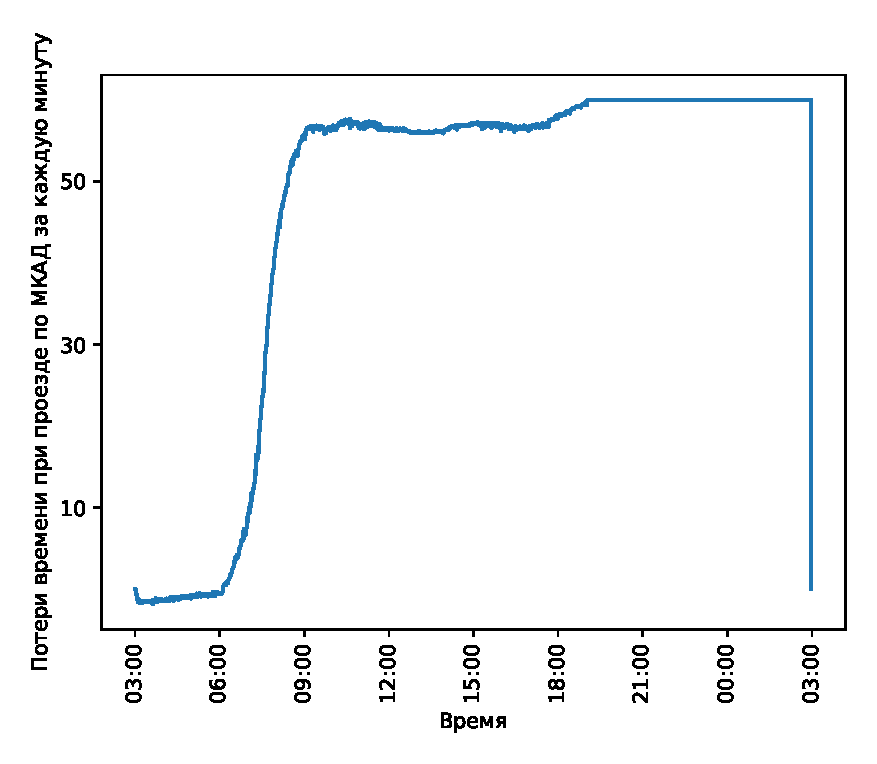
\includegraphics[width=1\linewidth]{MCAR_full_woenters_12_two_types_110_24h_3h_6km_Time_to_pass.eps}  \\ а) Без управления въездами
    \end{minipage}
    \hfill
    \begin{minipage}[b]{.49\textwidth}
        \centering
        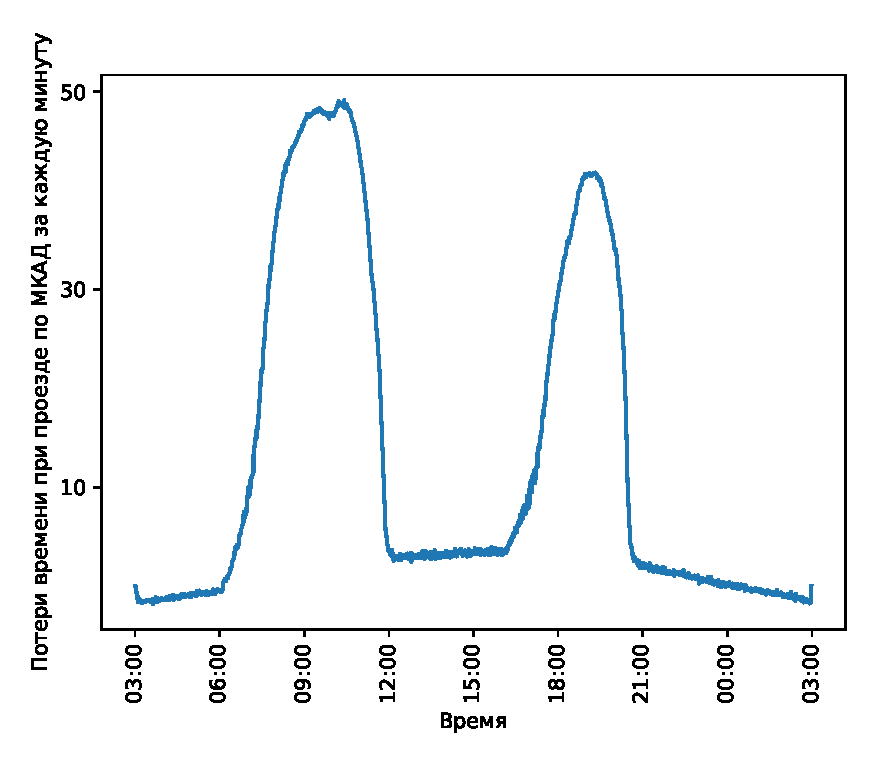
\includegraphics[width=1\linewidth]{MCAR_full_woenters_12_two_types_110_24h_3h_6km_handcontrol_Time_to_pass.eps}  \\ b) С управлением въездами
    \end{minipage}
    \hfill
    Временные потери на проезд по МКАД относительно пустой автомагистрали
\end{frame}


\subsection{Моделирование МКАД с вычислением всех фундаментальных диаграмм}
\begin{frame}[plain, noframenumbering]
    \begin{center}
        \Huge
        Моделирование МКАД с вычислением всех фундаментальных диаграмм
    \end{center}
\end{frame}
\begin{frame}
    \frametitle{Число автомобилей на автомагистрали}
    \centering
    \begin{minipage}[b]{0.49\textwidth}
        \centering
        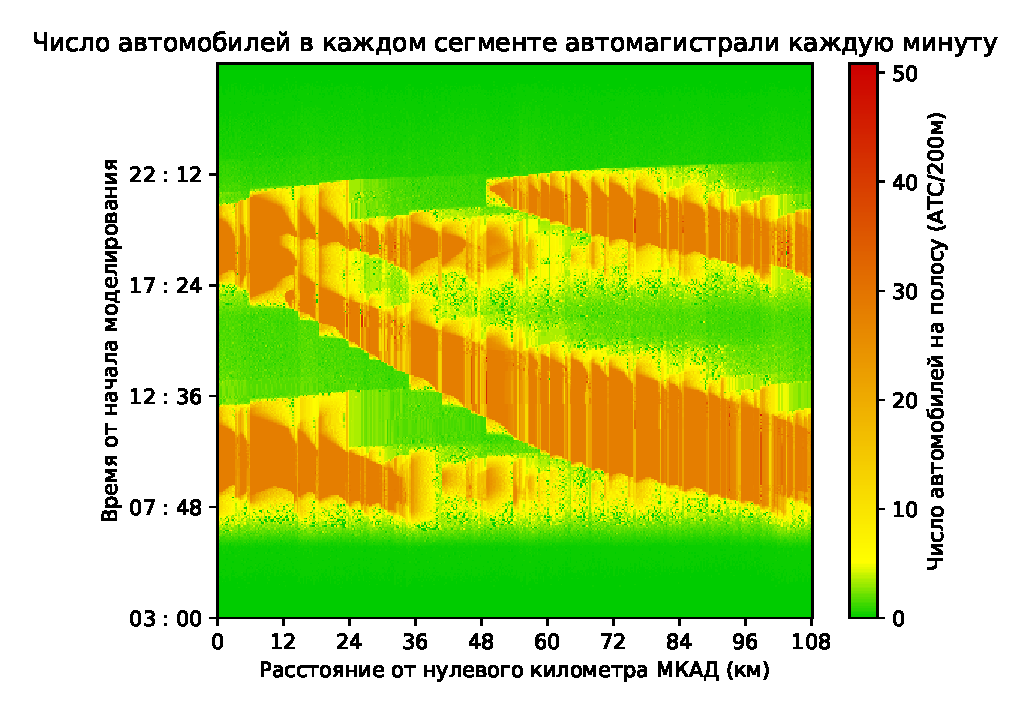
\includegraphics[width=1\linewidth]{MCAR_full_woenters_12_two_types_110_24h_3h_fullFD.eps}  \\ а) Без управления въездами
    \end{minipage}
    \hfill
    \begin{minipage}[b]{0.49\textwidth}
        \centering
        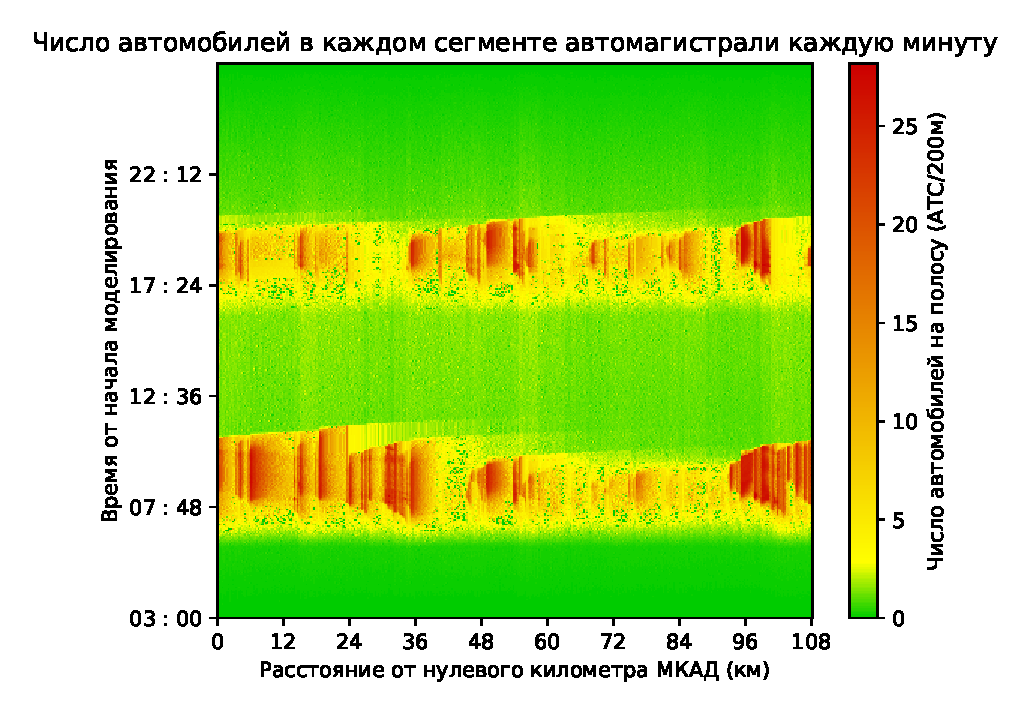
\includegraphics[width=1\linewidth]{MCAR_full_woenters_12_two_types_110_24h_3h_fullFD_handcontrol.eps}  \\ b) С управлением въездами
    \end{minipage}
    \hfill
    Количество автомобилей на 200 метров в модели транспортной сети МКАД за день
\end{frame}


\begin{frame}
    \frametitle{Число въехавших автомобилей}
    \centering
    \begin{minipage}[b]{.49\textwidth}
        \centering
        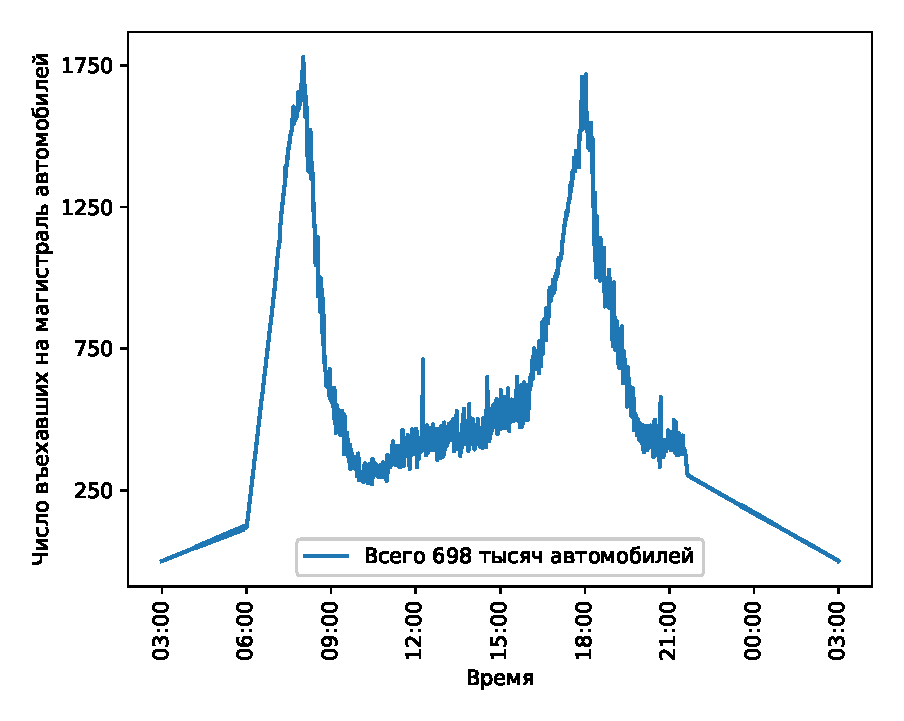
\includegraphics[width=1\linewidth]{MCAR_full_woenters_12_two_types_110_24h_3h_fullFD_Entered.eps}  \\ а) Без управления въездами
    \end{minipage}
    \hfill
    \begin{minipage}[b]{.49\textwidth}
        \centering
        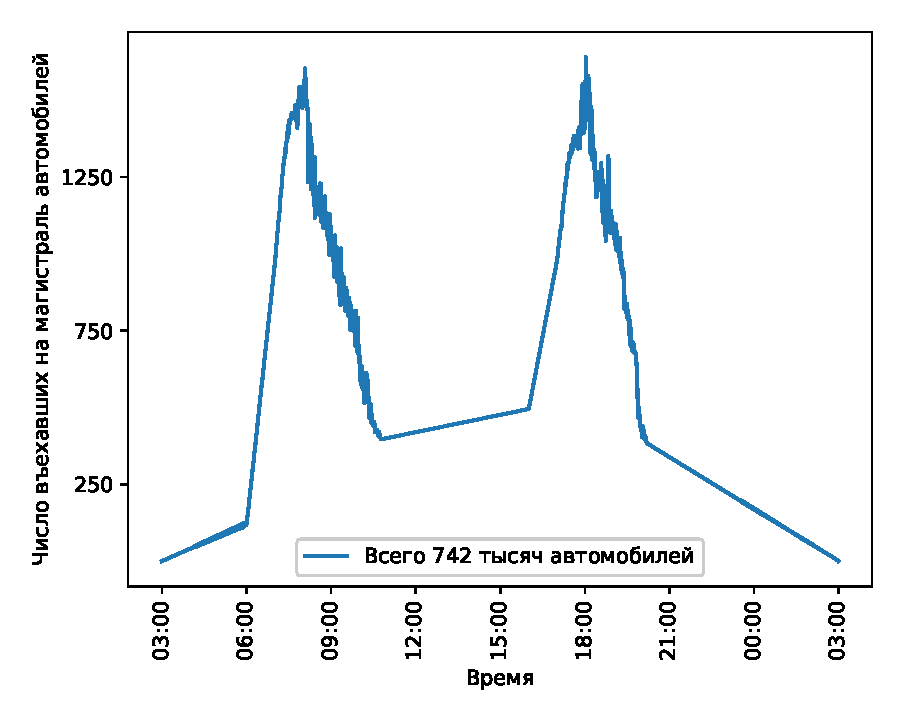
\includegraphics[width=1\linewidth]{MCAR_full_woenters_12_two_types_110_24h_3h_fullFD_handcontrol_Entered.eps}  \\ b) С управлением въездами
    \end{minipage}
    \hfill
    Графики суммарно въехавшего на МКАД со всех въездов числа автомобилей
\end{frame}


\begin{frame}
    \frametitle{Временные потери на проезд по МКАД}
    \centering
    \begin{minipage}[b]{.49\textwidth}
        \centering
        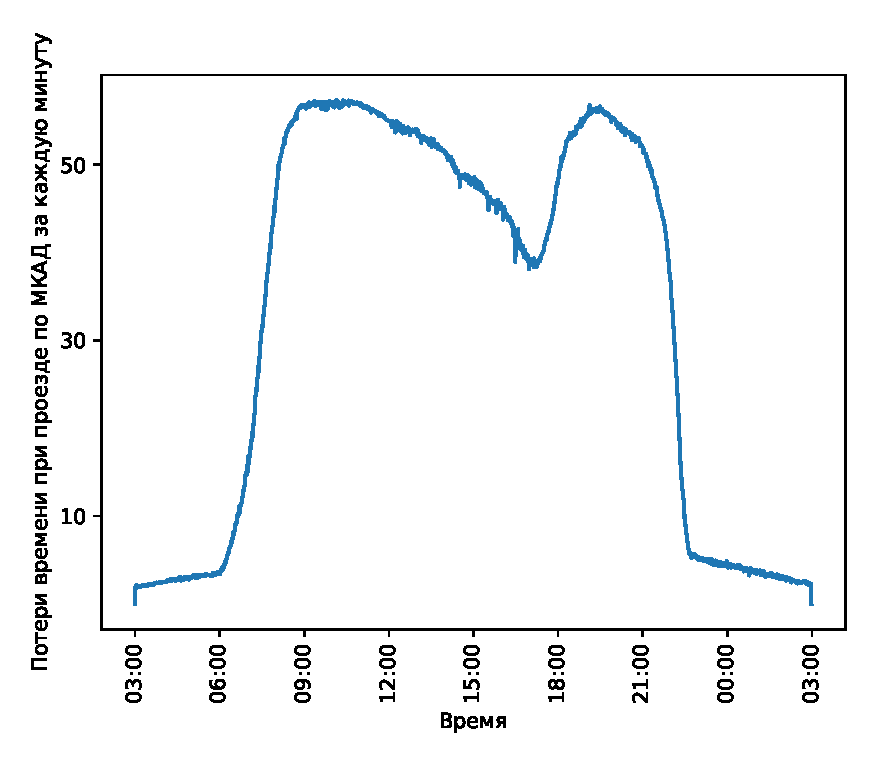
\includegraphics[width=1\linewidth]{MCAR_full_woenters_12_two_types_110_24h_3h_fullFD_Time_to_pass.eps}  \\ а) Без управления въездами
    \end{minipage}
    \hfill
    \begin{minipage}[b]{.49\textwidth}
        \centering
        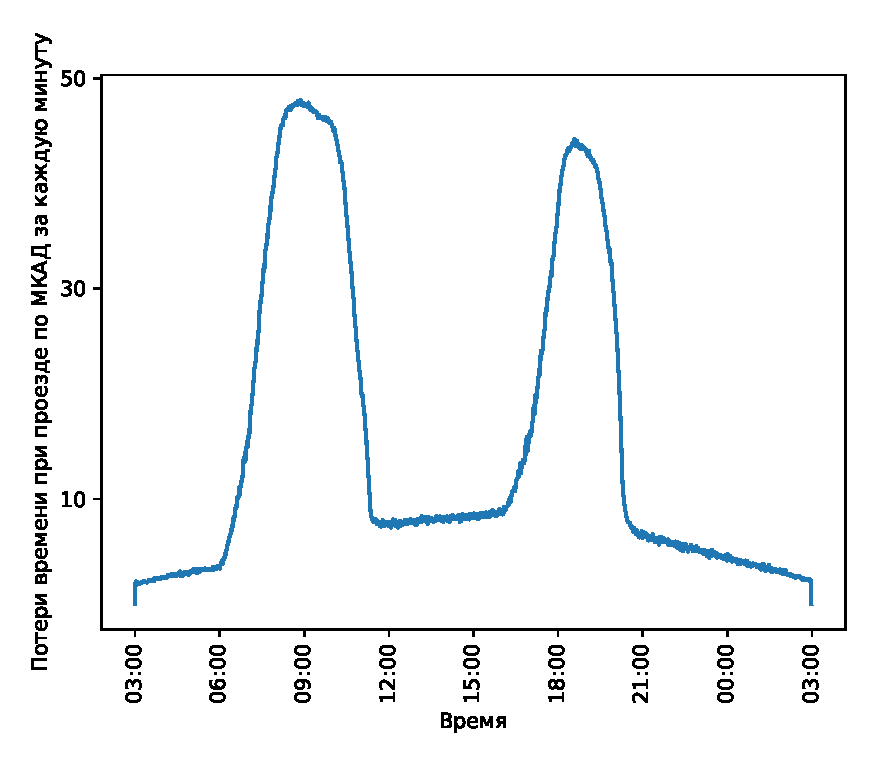
\includegraphics[width=1\linewidth]{MCAR_full_woenters_12_two_types_110_24h_3h_fullFD_handcontrol_Time_to_pass.eps}  \\ b) С управлением въездами
    \end{minipage}
    \hfill
    Временные потери на проезд по МКАД относительно пустой автомагистрали
\end{frame}

\subsection{Сравнение с моделью интеллектуального водителя}
\begin{frame}[plain, noframenumbering]
    \begin{center}
        \Huge
        Сравнение с моделью интеллектуального водителя (IDM)
    \end{center}
\end{frame}


\begin{frame}
    \frametitle{Моделирование небольшого участка автомагистрали}
    \centering
    \begin{minipage}[b]{0.49\textwidth}
        \centering
        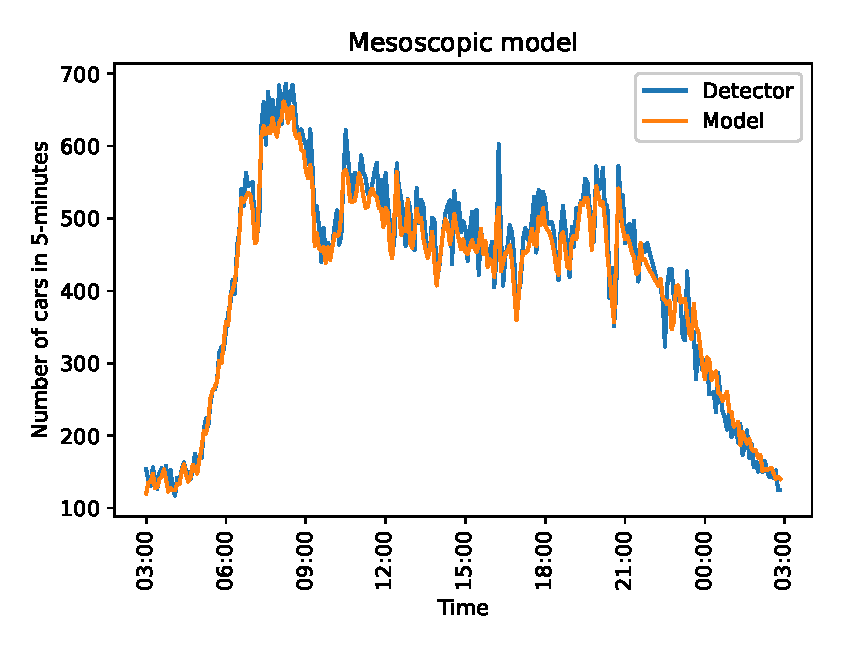
\includegraphics[width=1\linewidth]{simple_road_meso.eps}  \\ а) Результаты моделирования мезоскопической моделью
    \end{minipage}
    \hfill
    \begin{minipage}[b]{0.49\textwidth}
        \centering
        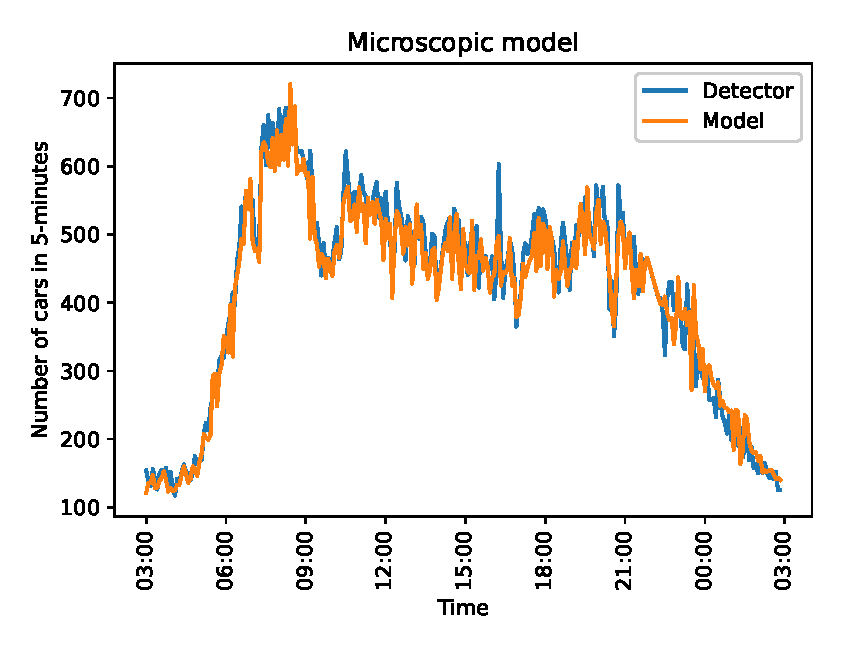
\includegraphics[width=1\linewidth]{simple_road_micro.eps}  \\ b) Результаты моделирования микроскопической моделью
    \end{minipage}
    \hfill
    Средняя относительная процентная ошибка (mean absolute percentile error - MAPE) для предложенной модели составила 5.35\%, для микроскопической модели составила 5.6\%.
    Ошибка предложенной модели относительно модели разумного водителя~- 1.7\%.
\end{frame}

\begin{frame}
    \frametitle{Моделирование небольшого участка автомагистрали}
    \centering
    \begin{minipage}[b]{.49\textwidth}
        \centering
        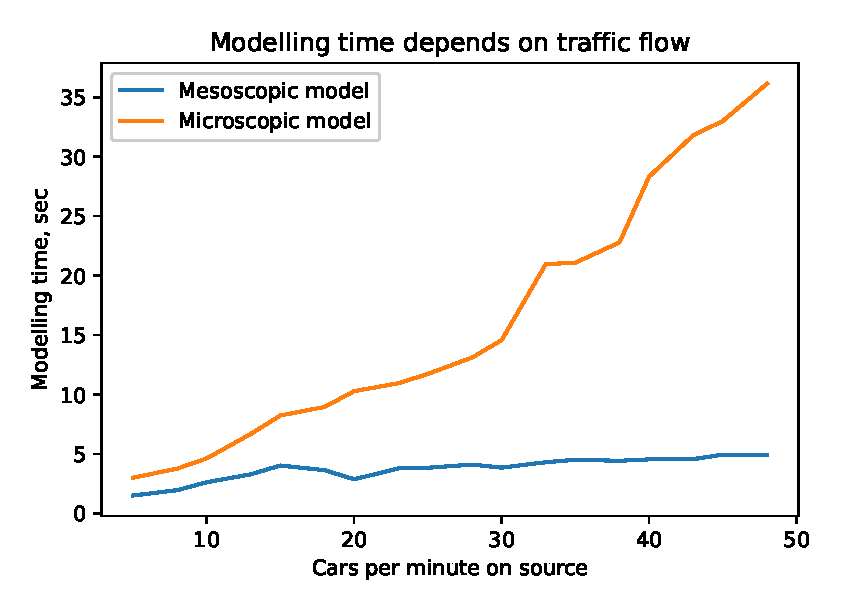
\includegraphics[width=1\linewidth]{modelling_time_cars.eps}  \\ а) Время моделирования в зависимости от потока АТС на въезде
    \end{minipage}
    \hfill
    \begin{minipage}[b]{.49\textwidth}
        \centering
        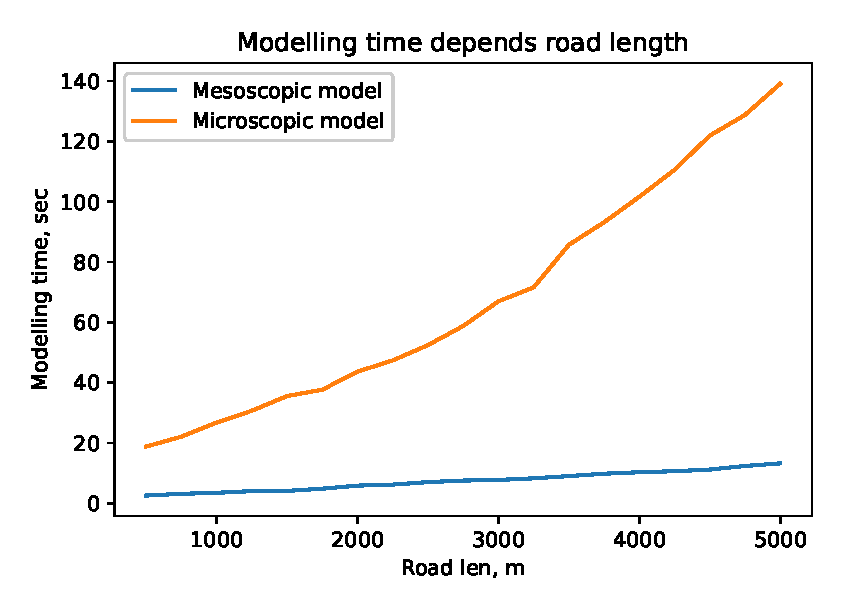
\includegraphics[width=1\linewidth]{modelling_time_length.eps}  \\ b) Время моделирования в зависимости от длины участка магистрали
    \end{minipage}
    \hfill
    Время моделирования моделями в зависимости от параметров потока АТС на въезде и длины моделируемого участка магистрали.
\end{frame}


\begin{frame}
    \frametitle{Результаты моделирования МКАД}
    \centering
    \begin{minipage}[b]{.53\textwidth}
        \centering
        \includegraphics[width=1\linewidth]{result.eps}  \\ а) Результаты моделирования мезоскопической моделью
    \end{minipage}
    \hfill
    \begin{minipage}[b]{.45\textwidth}
        \centering
        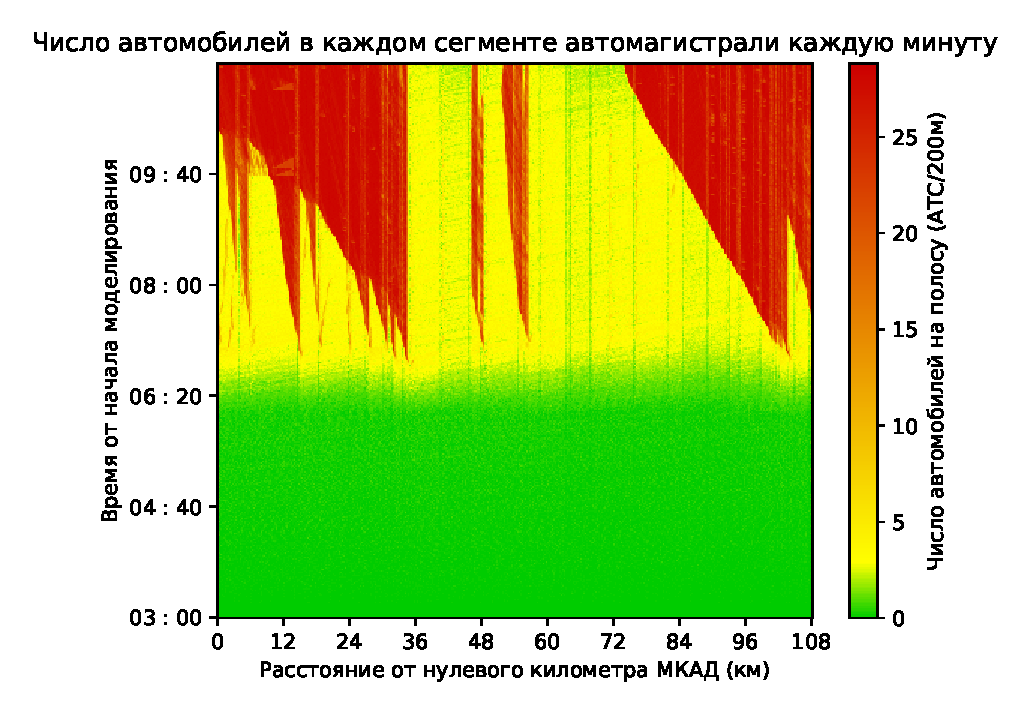
\includegraphics[width=1\linewidth]{MCAR_full_woenters_12_two_types_60_24h_3hmax_fullFD_micro_idm.eps}  \\ b) Результаты моделирования микроскопической моделью
    \end{minipage}
    \hfill
    Результаты моделирования всей автомагистрали двумя моделями. Средняя абсолютная процентная ошибка - 5.4\%.
    Ошибка определения режима - 2.8\%.
\end{frame}


% [plain, noframenumbering]
       % Настройки заглавной странице
\begin{frame}
    \frametitle{Научная новизна}
    \begin{itemize}
        \item Впервые была построена мезоскопическая модель на основе групп АТС с использованием фундаментальной диаграммы поток-плотность на основе комплексированных данных.
        \item Проведено исследование на адекватность моделирования на модельных и реальных данных.
        \item Было выполнено оригинальное исследование о применимости предложенной модели к адаптивному управлению выделенной автомагистрали с целью потенциального увеличения её пропускной способности.
        \item Предложен алгоритм комплексирования данных с дорожных датчиков и GPS-треков.
    \end{itemize}
\end{frame}
\note{
    Проговаривается вслух научная новизна
}

\begin{frame}[t,allowframebreaks] % публикации на одной странице
% \begin{frame}[t,allowframebreaks] % публикации на нескольких страницах
    \frametitle{Основные публикации}
    \nocite{star2016compl}%
    \nocite{star2017ident}%
    \nocite{star2021adaptcontrol}%
    \nocite{star2021statmod}%
    \nocite{collectiveArticle2}%
    \nocite{alekseenko2017adaptive}%
    %
    %% authorwos
    \nocite{wosbib1}%
    %
    %% authorscopus
    \nocite{scbib1}%
    %
    %% authorconf
    \nocite{confbib1}%
    \nocite{confbib2}%
    %
    %% authorother
    \nocite{bib1}%
    \nocite{bib2}%
    \ifnumequal{\value{bibliosel}}{0}{
        \insertbiblioauthor
    }{
        \printbibliography%
    }
\end{frame}
\note{
    Результаты работы опубликованы в N печатных изданиях,
    в~т.\:ч. M реферируемых изданиях.
}

\begin{frame}
    \frametitle{Участие в конференциях}
    \begin{itemize}
        \item 11-я Международная конференция «Интеллектуализация обработки информации», 2016;
        \item 18-я Всероссийская конференция с международным участием «Математические методы распознавания образов», 2017;
        \item 19-я Всероссийская конференция с международным участием «Математические методы распознавания образов», 2019;
        \item XXVII Международной конференции студентов, аспирантов и молодых учёных «Ломоносов», 2020;
        \item 13-я Международная конференция «Интеллектуализация обработки информации», 2020;
        \item XXVIII Международной конференции студентов, аспирантов и молодых учёных «Ломоносов», 2020;
        \item 20-я Всероссийская конференция с международным участием «Математические методы распознавания образов», 2021;
    \end{itemize}
\end{frame}
\note{
    Работа была представлена на ряде конференций.
}

\begin{frame}[plain, noframenumbering] % последний слайд без оформления
    \begin{center}
        \Huge
        Спасибо за внимание!
    \end{center}
\end{frame}
    % Последние слайды презентации
\appendix
% \begin{frame}
    \frametitle{Ответы на замечания ведущей организации НИИ~<<\dots>>}
    \begin{itemize}
        \item Замечание -- ответ
        \item Замечание -- ответ
        \item Замечание -- ответ
        \item Замечание -- ответ
        \item Замечание -- ответ
    \end{itemize}
\end{frame}

\begin{frame}
    \frametitle{Ответы на замечания оф. оппонента Иванова\,И.\,И}
    \begin{itemize}
        \item Замечание -- ответ
        \item Замечание -- ответ
        \item Замечание -- ответ
        \item Замечание -- ответ
        \item Замечание -- ответ
    \end{itemize}
\end{frame}

\begin{frame}
    \frametitle{Ответы на замечания Петрова\,П.\,П}
    \begin{itemize}
        \item Замечание -- ответ
        \item Замечание -- ответ
        \item Замечание -- ответ
        \item Замечание -- ответ
        \item Замечание -- ответ
    \end{itemize}
\end{frame}
      % Запасные слайды презентации
\end{document}
